\subsection{Definition of regular local rings}

Let A be a Noetherian local ring. Let \((x_{i})_{i\in I}\) be a family of elements of \(m_{A}\) . According to cor. 2 of prop. 4 of II, § 3, n° 2, it is equivalent to suppose that the family \((x_{i})_{i\in I}\) generates the ideal \(m_{A}\) of A, or that the classes of the \(x_{i}\) modulo \(m_{A}^{2}\) generate the \(\kappa_{A}\) -vector space \(m_{A}/m_{A}^{2}\) ; if this is so, one has dim(A) ≤ Card(I) by the scholium of § 3, n° 2. One therefore has the inequality

\[
\dim (A) \leqslant [ m _ {A} / m _ {A} ^ {2}: \kappa_ {A} ] \leqslant \operatorname{Card} (I)\tag{1}
\]

for every family \((x_{i})_{i\in I}\) generating the ideal \(m_{A}\) of A.

DEFINITION 1. --- The Noetherian local ring A is said to be regular if one has \(\dim(A) = [m_A/m_A^2:\kappa_A]\). One then calls a system of coordinates of A every family of elements of \(m_A\) whose classes modulo \(m_A^2\) form a basis of the \(\kappa_A\)-vector space \(m_A/m_A^2\).

A system of coordinates in a regular Noetherian local ring A is therefore a finite family \((x_{i})_{i\in I}\) generating the ideal \(m_{A}\) of A and such that \(\text{Card}(I) = \dim(A)\) . Conversely, if the ideal \(m_{A}\) of a Noetherian local ring A is generated by d elements with \(d \leqslant \dim(A)\) , the ring A is regular.

Examples. --- 1) The regular Noetherian local rings of dimension 0 (resp. 1) are the fields (resp. the discrete valuation rings) (VI, § 3, n° 6, prop. 9 and cor. 1 of th. 1 below). Let A be a discrete valuation ring; then an element t of m \(_{A}\) is a uniformizer if and only if \{t\} is a system of coordinates of A.

\begin{enumerate}
\def\labelenumi{\arabic{enumi})}
\setcounter{enumi}{1}
\tightlist
\item
  Let \(k\) be a field and let \(n\) be a positive integer. The ring of formal power series \(k[[X_1, ..., X_n]]\) is a regular Noetherian local ring of dimension \(n\) (§ 3, n° 4, cor. 3 of prop. 8). Let \(F_1, ..., F_n\) be formal power series without constant term in \(k[[X_1, ..., X_n]]\) ; for the sequence \((F_1, ..., F_n)\) to be a system of coordinates of \(k[[X_1, ..., X_n]]\) , it is necessary and sufficient that the matrix \(\left(\frac{\partial F_i}{\partial X_j}(0, ..., 0)\right)\) be invertible.
\end{enumerate}

More generally, let A be a regular Noetherian local ring of dimension \(r\) ; then \(A[[X_1, ..., X_n]]\) is a regular Noetherian local ring of dimension \(r + n\) . If \((a_1, ..., a_r)\) is a system of coordinates of A, then \((a_1, ..., a_r, X_1, ..., X_n)\) is a system of coordinates of \(A[[X_1, ..., X_n]]\) .

\begin{enumerate}
\def\labelenumi{\arabic{enumi})}
\setcounter{enumi}{2}
\tightlist
\item
  Let A be a complete regular Noetherian local ring of dimension \(r\) . The ring A \(\{X_1, ..., X_n\}\) of restricted formal power series is a regular Noetherian local ring of dimension \(r + n\) (§ 3, n° 4, remark 1). If \((a_1, ..., a_r)\) is a system of coordinates of A, then \((a_1, ..., a_r, X_1, ..., X_n)\) is a system of coordinates of A \(\{X_1, ..., X_n\}\) .
\end{enumerate}

* 4) Let \(k\) be a complete non-discrete valued field. The ring of formal power series in \(n\) variables which converge in a neighborhood of 0 in \(k^n\) is a regular Noetherian local ring of dimension \(n\) ( \(\S\) 3, n° 4, remark 2). *

\begin{enumerate}
\def\labelenumi{\arabic{enumi})}
\setcounter{enumi}{4}
\tightlist
\item
  Let \(k\) be a field, A a \(k\) -algebra of finite type which is an integral domain, and \(\mathfrak{m}\) a maximal ideal of A. The Noetherian local ring \(\mathrm{A}_{\mathfrak{m}}\) is regular if and only if one has \(\dim(\mathrm{A}) = [\mathfrak{m}/\mathfrak{m}^{2}:\mathrm{A}/\mathfrak{m}]\) : indeed, one has \(\dim(\mathrm{A}_{\mathfrak{m}}) = \dim(\mathrm{A})\) ( \(\S 2\) , \(no. 4\) , cor. 2 of th. 3) and the vector spaces \(\mathfrak{m}/\mathfrak{m}^{2}\) and \(\mathrm{mA}_{\mathfrak{m}}/(\mathrm{mA}_{\mathfrak{m}})^{2}\) over the field A/m are isomorphic (II, \(\S 3\) , \(no. 3\) , prop. 9). In particular, if \(k\) is algebraically closed, the stated condition is equivalent to \(\dim(\mathrm{A}) = [\mathfrak{m}/\mathfrak{m}^{2}:k]\) (V, \(\S 3\) , \(no. 3\) , prop. 1).
\end{enumerate}

* 6) Let X be an algebraic variety over a perfect field \(k\) . Then X is nonsingular at a point \(x\) if and only if the local ring of X at \(x\) is regular. *

* 7) Let A be a regular Noetherian local ring. It will be seen later that the Noetherian local ring \(A_{p}\) is regular for every prime ideal p of A. *

PROPOSITION 1.--- Let A and B be Noetherian local rings and \(\rho:A\to B\) a local homomorphism making B a flat A-module. Suppose that one has \(m_{B} = B \cdot \rho(m_{A})\) . Then one has \(\dim(A) = \dim(B)\) and B is regular if and only if A is regular.

The first assertion follows from cor. 1 of prop. 7 of § 3, no. 4. Since B is flat over A, one may identify \(\mathfrak{m}_{\mathrm{B}}^{k} = \mathbf{B}.\rho (\mathfrak{m}_{\mathrm{A}}^{k})\) with \(\mathbf{B}\otimes_{\mathbf{A}}\mathfrak{m}_{\mathbf{A}}^{k}\) for every integer \(k\geqslant 0\) , hence \(\mathfrak{m}_{\mathrm{B}} / \mathfrak{m}_{\mathrm{B}}^{2}\) with \(\mathbf{B}\otimes_{\mathbf{A}}(\mathfrak{m}_{\mathrm{A}} / \mathfrak{m}_{\mathrm{A}}^{2})\) or again with \(\kappa_{\mathrm{B}}\otimes_{\kappa_{\mathrm{A}}}(\mathfrak{m}_{\mathrm{A}} / \mathfrak{m}_{\mathrm{A}}^{2})\) . One therefore has

\[
\left[ \mathfrak {m} _ {\mathrm{B}} / \mathfrak {m} _ {\mathrm{B}} ^ {2}: \kappa_ {\mathrm{B}} \right] = \left[ \mathfrak {m} _ {\mathrm{A}} / \mathfrak {m} _ {\mathrm{A}} ^ {2}: \kappa_ {\mathrm{A}} \right],\tag{2}
\]

whence the proposition immediately.

COROLLARY. --- A Noetherian local ring A is regular if and only if its completion \(\hat{A}\) is.

Indeed, \(\hat{\mathbf{A}}\) is flat over \(\mathbf{A}\) , and one has \(\mathfrak{m}_{\hat{\mathbf{A}}} = \hat{\mathbf{A}}. \mathfrak{m}_{\mathbf{A}}\) (III, § 3, no. 4, th. 3 and § 2, no. 12, cor. 2 to prop. 16).

\subsection{Graded ring associated with a regular local ring}

THEOREM 1. --- Let A be a Noetherian local ring. The following conditions are equivalent:

\begin{enumerate}
\def\labelenumi{(\roman{enumi})}
\item
  A is regular.
\item
  The ideal \(\mathfrak{m}_{\mathbf{A}}\) is generated by a secant subset for A (§ 3, no. 2, def. 1).
\item
  The ideal \(\mathfrak{m}_{\mathrm{A}}\) is generated by a completely secant sequence for A (A, X, p.~157, def. 2).
\item
  Let S be the symmetric algebra of the \(\kappa_{\mathbf{A}}\) -vector space \(\mathfrak{m}_{\mathbf{A}} / \mathfrak{m}_{\mathbf{A}}^{2}\) , and let \(\operatorname{gr}(\mathbf{A}) = \bigoplus_{n \geqslant 0} \mathfrak{m}_{\mathbf{A}}^{n} / \mathfrak{m}_{\mathbf{A}}^{n+1}\) be the graded ring associated with A. The canonical homomorphism \(\gamma\) of S onto \(\operatorname{gr}(\mathbf{A})\) is bijective
\item
  There exists an integer \(r \geqslant 0\) such that one has \(H_{\mathbf{A},\mathfrak{m}_{\mathbf{A}}} = (1 - \mathrm{T})^{-r}\) , that is, \(\mathfrak{m}_{\mathbf{A}} = 0\) if \(r = 0\) and \([\mathfrak{m}_{\mathbf{A}}^{n}/\mathfrak{m}_{\mathbf{A}}^{n+1}:\kappa_{\mathbf{A}}] = \binom{n + r - 1}{r - 1}\) for every integer \(n \geqslant 0\) if \(r > 0\) .
\item
  We have \(\mathrm{H}_{\mathrm{A},\mathfrak{m}_{\mathrm{A}}} = (1 - \mathrm{T})^{-d}\) with \(d = \dim (\mathrm{A})\)
\end{enumerate}

If these conditions are satisfied, every system of coordinates of A is a completely secant sequence for A.

\begin{enumerate}
\def\labelenumi{(\roman{enumi})}
\setcounter{enumi}{1}
\item
  \(\Rightarrow\) (i): indeed, every secant subset has at most dim(A) elements ( \(\S 3\) , no. 2, th. 1).
\item
  \(\Rightarrow\) (ii): indeed, every completely secant sequence is secant (§ 3, no. 2, corollary of prop. 3).
\end{enumerate}

\((\mathrm{iv}) \Rightarrow (\mathrm{iii}) : \text{let } (x_1, ..., x_r)\) be a sequence of elements of \(\mathfrak{m}_{\mathbf{A}}\) whose classes modulo \(\mathfrak{m}_{\mathbf{A}}^2\) form a basis \((\xi_1, ..., \xi_r)\) of \(\mathfrak{m}_{\mathbf{A}} / \mathfrak{m}_{\mathbf{A}}^2\) over the field \(\kappa_{\mathbf{A}}\) . If property (iv) is satisfied, \(\operatorname{gr}(\mathbf{A})\) is the polynomial algebra \(\kappa_{\mathbf{A}}[\xi_1, ..., \xi_r]\) and the sequence \((x_1, ..., x_r)\) is completely secant (A, X, p.~160, th. 1). This also proves the last assertion of th. 1.

\begin{enumerate}
\def\labelenumi{(\roman{enumi})}
\tightlist
\item
  \(\Rightarrow\) (iv): set \(r = [\mathfrak{m}_{\mathbf{A}} / \mathfrak{m}_{\mathbf{A}}^{2}:\kappa_{\mathbf{A}}]\) . According to formula (6) of § 4, no. 2, the Poincaré series of the graded vector space S over the field \(\kappa_{\mathbf{A}}\) is equal to
\end{enumerate}

\[
\mathrm{P} _ {\mathrm{S}} = \sum_ {n \geqslant 0} \left[ \mathrm{S} ^ {n} (\mathfrak {m} _ {\mathrm{A}} / \mathfrak {m} _ {\mathrm{A}} ^ {2}): \kappa_ {\mathrm{A}} \right] \mathrm{T} ^ {n} = (1 - \mathrm{T}) ^ {- r}.
\]

Suppose that the canonical homomorphism \(\gamma: S \to \mathrm{gr}(A)\) is not bijective. Since \(\gamma\) is surjective, there exists a homogeneous element \(u\) of \(S\) , of degree \(d > 0\) , annihilated by \(\gamma\) . Then one has

\[
\begin{array}{r l} \mathrm {H_ {A,m_ {A}}} = & \mathrm {P_ {S}} - \symrm {P_ {Ker(\gamma)}} \leqslant \mathrm {P_ {S}} - \mathrm {P_ {uS}} = (1 - \mathrm{T} ^ {d}) / (1 - \mathrm{T}) ^ {r} = \\ & = (1 + \mathrm{T} + \dots + \mathrm{T} ^ {d - 1}) / (1 - \mathrm{T}) ^ {r - 1}. \end{array}
\]

According to th. 3 of § 4, no. 4 and lemma 2 of § 4, no. 1, one therefore has dim(A) \textless{} r, and A is not regular.

Let us finally prove the equivalence of conditions (iv) through (vi). Now, (iv) means that we have \(\mathrm{H}_{\mathrm{A},\mathfrak{m}_{\mathrm{A}}}=(1-\mathrm{T})^{-s}\) with \(s=[\mathfrak{m}_{\mathrm{A}}/\mathfrak{m}_{\mathrm{A}}^{2}:\kappa_{\mathrm{A}}]\). Therefore conditions (iv), (v), (vi) mean that we have \(\mathrm{H}_{\mathrm{A},\mathfrak{m}_{\mathrm{A}}}=(1-\mathrm{T})^{-m}\) , with respectively \(m=[\mathfrak{m}_{\mathrm{A}}/\mathfrak{m}_{\mathrm{A}}^{2}:\kappa_{\mathrm{A}}]\) , \(m\geqslant0\) , \(m=\dim(\mathrm{A})\). But if one has \(\mathrm{H}_{\mathrm{A},\mathfrak{m}_{\mathrm{A}}}=(1-\mathrm{T})^{-m}\) , one has \(\dim(\mathrm{A})=m\) by §4, no. 4, th. 3 and \([\mathfrak{m}_{\mathrm{A}}/\mathfrak{m}_{\mathrm{A}}^{2}:\kappa_{\mathrm{A}}]=m\) (since \((1-\mathrm{T})^{-m}=1+m\mathrm{T}+\cdots\) ). The equivalence of conditions (iv) to (vi) follows immediately.

COROLLARY 1. --- Every regular Noetherian local ring is integrally closed, and in particular an integral domain.

Assume A is regular. Then gr(A) is isomorphic to a polynomial algebra in finitely many indeterminates over a field (th. 1, (iv)). Consequently, gr(A) is a Noetherian integrally closed ring (V, § 1, no. 3, cor. 3 of prop. 13), and hence A is integrally closed (V, § 1, no. 4, prop. 15).

We shall see in a later chapter that every regular Noetherian local ring is factorial.

COROLLARY 2.---Let A and B be Noetherian local rings and σ a local homomorphism from B to A. Suppose A is regular and B is complete. For σ to be bijective, it is necessary and sufficient that it induce bijections of κ \(_{B}\) on κ \(_{A}\) and of m \(_{B}\) /m \(_{B}^{2}\) on m \(_{A}\) /m \(_{A}^{2}\) .

The stated condition is obviously necessary.

Suppose conversely that \(\sigma\) induces isomorphisms of \(\mathrm{gr}_{0}(\mathbf{B})\) onto \(\mathrm{gr}_{0}(\mathbf{A})\) and of \(\mathrm{gr}_{1}(\mathbf{B})\) onto \(\mathrm{gr}_{1}(\mathbf{A})\). Since the ring \(\mathrm{gr}(\mathbf{B})\) is generated by \(\mathrm{gr}_{0}(\mathbf{B}) \cup \mathrm{gr}_{1}(\mathbf{B})\) and that \(\mathrm{gr}(\mathbf{A})\) is the symmetric algebra of the vector space \(\mathrm{gr}_{1}(\mathbf{A})\) over the field \(\mathrm{gr}_{0}(\mathbf{A})\) , the homomorphism \(\mathrm{gr}(\sigma)\) is bijective. Consequently, \(\sigma\) is bijective (III, § 2, no. 8, cor. 3 of th. 1).

COROLLARY 3. --- Let \(k\) be a field and A a local Noetherian \(k\)-algebra, whose residue field is equal to \(k\). For A to be regular, it is necessary and sufficient that its completion \(\hat{A}\) be isomorphic to a \(k\)-algebra of formal series \(k[[X_1, ..., X_n]]\) .

This follows from the equivalence of (i) and (iv) in Thm. 1, and from Prop. 11 of III, § 2, no. 9.

\subsection{Quotients of regular local rings}

PROPOSITION 2. --- Let A be a Noetherian local ring, \(\boldsymbol{x} = (x_1, ..., x_r)\) a sequence of elements of \(\mathfrak{m}_{\mathrm{A}}\) and \(\mathfrak{x}\) is the ideal generated by \(\boldsymbol{x}\). The following conditions are equivalent:

\begin{enumerate}
\def\labelenumi{(\roman{enumi})}
\item
  the ring A is regular, and x is part of a coordinate system of A;
\item
  the ring A/x is regular and x is a secant sequence for A ;
\item
  the ring A/x is regular and x is a completely secant sequence for A.
\end{enumerate}

Moreover, when these conditions are satisfied, x is a prime ideal of A.

\begin{enumerate}
\def\labelenumi{(\roman{enumi})}
\setcounter{enumi}{2}
\item
  \(\Rightarrow\) (ii): this follows from the corollary of Prop. 3 in § 3, no. 2.
\item
  \(\Rightarrow\) (i): suppose that \(x\) is a secant sequence for A and that the Noetherian local ring A/\(x\) is regular. Let \((x_{r+1}, ..., x_d)\) be a sequence of elements of A, whose classes modulo \(x\) form a system of coordinates of A/\(x\). Then the sequence \((x_1, ..., x_d)\) generates the ideal \(m_A\) of A, and we have
\end{enumerate}

\[
\dim (\mathrm{A}) = r + \dim (\mathrm{A} / \mathrm{x}) = r + (d - r) = d.
\]

Consequently, A is regular and \((x_{1},\ldots,x_{d})\) is a system of coordinates of A.

\begin{enumerate}
\def\labelenumi{(\roman{enumi})}
\tightlist
\item
  \(\Rightarrow\) (iii): if condition (i) is satisfied, the sequence \(x\) is completely secant (no. 2, th. 1), hence secant by the corollary of prop. 3 of § 3, no. 2. We therefore have
\end{enumerate}

\[
\dim (\mathrm{A} / \mathfrak {x}) = \dim (\mathrm{A}) - r;\tag{3}
\]

moreover, the classes of \(x_{1},\ldots,x_{r}\) modulo \(\mathfrak{m}_{\mathbf{A}}^{2}\) are linearly independent over the field \(\kappa_{\mathbf{A}}\) , and we therefore have

\[
\left[ \mathfrak {m} _ {\mathrm{A}} / (\mathfrak {m} _ {\mathrm{A}} ^ {2} + x): \kappa_ {\mathrm{A}} \right] = \left[ \mathfrak {m} _ {\mathrm{A}} / \mathfrak {m} _ {\mathrm{A}} ^ {2}: \kappa_ {\mathrm{A}} \right] - r.\tag{4}
\]

Formulas (3) and (4) show that A/x is regular.

Every regular Noetherian local ring is an integral domain by Cor. 1 of Th. 1 of No. 2. Consequently, x is prime if A/x is regular.

COROLLARY 1. --- Let A be a Noetherian local ring, and let t be an element of \(\mathfrak{m}_{\mathrm{A}}\). The following conditions are equivalent:

\begin{enumerate}
\def\labelenumi{(\roman{enumi})}
\item
  A is regular, and t does not belong to \(m_{A}^{2}\) ;
\item
  A/tA is regular and \(\dim(\mathrm{A}/t\mathrm{A}) < \dim(\mathrm{A})\) ;
\item
  A/tA is regular, and t is not a zero divisor in A.
\end{enumerate}

COROLLARY 2. --- Let A be a regular Noetherian local ring, and let q be an ideal of A. Then A/q is regular if and only if q is generated by a subset of a system of coordinates of A.

The condition is sufficient by Prop. 2.

Suppose A/q is regular, and let \(x = (x_{1}, \ldots, x_{r})\) be a sequence of elements of q whose classes modulo \(m_{A}^{2}\) form a basis of \((\mathfrak{q} + \mathfrak{m}_{\mathrm{A}}^{2})/\mathfrak{m}_{\mathrm{A}}^{2}\) over the field \(\kappa_{A}\). Let x be the ideal of A generated by x. We therefore have \(x \subset q\) and x is part of a system of coordinates of A, so the Noetherian local ring A/x is regular (prop. 2); moreover, the vector spaces \(\mathfrak{m}_{\mathrm{A}}/(\mathfrak{q} + \mathfrak{m}_{\mathrm{A}}^{2})\) and \(\mathfrak{m}_{\mathrm{A}}/(\mathfrak{x} + \mathfrak{m}_{\mathrm{A}}^{2})\) have the same dimension over \(\kappa_{A}\). Consequently, the regular Noetherian local rings A/q and A/x have the same dimension. Since the ideals q and x are prime and we have \(x \subset q\) , we finally have q = x.

Example. --- Let \(k\) be a field, \(\mathbf{A} = k[[\mathbf{X}_1, ..., \mathbf{X}_n]]\) and \(\mathfrak{q}\) an ideal of \(\mathbf{A}\) , distinct from \(\mathbf{A}\) . For \(\mathbf{A}/\mathfrak{q}\) to be regular, it is necessary and sufficient that one can find an integer \(r \geqslant 0\) and elements \(\mathbf{F}_1, ..., \mathbf{F}_r\) of \(\mathbf{A}\) , generating \(\mathfrak{q}\) , and such that the matrix \(\left(\frac{\partial\mathbf{F}_i}{\partial\mathbf{X}_j}(0, ..., 0)\right)\) be of rank \(r\) ("Jacobian criterion"). We then have \(\dim(\mathbf{A}/\mathfrak{q}) = n - r\) .

Remark. --- Let A be a regular Noetherian local ring and \(q \subset m_{A}\) an ideal of A such that A/q is regular. Let \((x_{1}, \ldots, x_{r})\) be a sequence of elements of q whose classes modulo \(m_{A}^{2}\) generate the vector space \((\mathfrak{q} + \mathfrak{m}_{\mathrm{A}}^{2}) / \mathfrak{m}_{\mathrm{A}}^{2}\) over the field \(\kappa_{A}\). The proof of cor. 2 shows that the ideal q of A is generated by \((x_{1}, \ldots, x_{r})\) .

\subsection{Eisenstein polynomials}

DEFINITION 2. --- Let A be a ring, p a prime ideal of A, and P a polynomial in A{[}T{]}. We say that P is an Eisenstein polynomial for p if it satisfies the following conditions:

\begin{enumerate}
\def\labelenumi{\alph{enumi})}
\item
  P is monic of degree \(d \geqslant 1\) ;
\item
  we have \(\mathrm{P(T)}\equiv \mathrm{T}^d\bmod \mathfrak{pA}[\mathrm{T}];\)
\item
  we have \(\mathbf{P}(0)\notin \mathfrak{p}^2\)
\end{enumerate}

In other words, an Eisenstein polynomial for p is a polynomial of the form \(\mathbf{P}(\mathbf{T}) = \mathbf{T}^{d} + \sum_{i=1}^{d} a_{i} \mathbf{T}^{d-i}\) , with \(d \geqslant 1\) , where \(a_{1}, \ldots, a_{d-1}\) belong to p and \(a_{d}\) lies in \(p - p^{2}\) .

We say that P is an Eisenstein polynomial for \(pA_{p}\) if the canonical image of P in the polynomial ring \(A_{p}[T]\) is an Eisenstein polynomial for the ideal \(pA_{p}\) ; this also means that P is an Eisenstein polynomial for p and that it satisfies in addition the following condition, stronger than c):

\(c^{\prime})\) every element \(a\) of A such that \(a\mathbf{P}(0)\in\mathfrak{p}^{2}\) belongs to \(\mathfrak{p}\) .

PROPOSITION 3. --- Let A be a ring, p a prime ideal of A, and P ∈ A{[}T{]} an Eisenstein polynomial for p.

\begin{enumerate}
\def\labelenumi{\alph{enumi})}
\item
  There is no decomposition of the form \(P = P_{1}P_{2}\) where \(P_{1}\) and \(P_{2}\) are two monic polynomials of A{[}T{]} distinct from 1.
\item
  Suppose A is integrally closed, with field of fractions K. Then P is irreducible in K[T].
\end{enumerate}

Let \(\varphi\) be the canonical homomorphism from A into the field of fractions \(k\) of A/p, and let \(\varphi':\mathrm{A}[\mathrm{T}]\to k[\mathrm{T}]\) be the extension of \(\varphi\) such that \(\varphi'(\mathrm{T})=\mathrm{T}\). Suppose we have \(\mathbf{P}=\mathbf{P}_{1}\mathbf{P}_{2}\) where \(\mathbf{P}_{1}\) and \(\mathbf{P}_{2}\) are two monic polynomials of A{[}T{]} distinct from 1. We then have \(\mathrm{T}^{d}=\varphi'(\mathbf{P}_{1})\varphi'(\mathbf{P}_{2})\) in \(k[\mathrm{T}]\) , denoting \(d\) the degree of P. If \(d_{i}\) is the degree of \(\mathbf{P}_{i}\) , one therefore has \(\varphi'(\mathbf{P}_{i})=\mathrm{T}^{d_{i}}\) , that is, \(\mathbf{P}_{i}(\mathrm{T})\equiv\mathrm{T}^{d_{i}}\text{ mod. pA[T]}\) , and in particular \(\mathbf{P}_{i}(0)\in\mathfrak{p}\) . But then \(\mathrm{P}(0)=\mathrm{P}_{1}(0).\mathrm{P}_{2}(0)\) belongs to \(\mathfrak{p}^{2}\) contrary to the hypotheses. This proves \(a\).

The assertion \(b)\) follows from \(a)\) and from prop. 11 of V, § 1, no. 3.

Let A be a Noetherian local ring and \(P_{1}, \ldots, P_{r}\) monic polynomials in A{[}T{]}, of degree \(\geqslant 2\). Let q be the ideal of A{[}T \(_{1}\) , \ldots, T \(_{r}\) {]} generated by \(\mathrm{P}_{1}(\mathrm{T}_{1}), \ldots, \mathrm{P}_{r}(\mathrm{T}_{r})\) and let B be the quotient A-algebra A{[}T \(_{1}\) , \ldots, T \(_{r}\) {]}/q. For \(1 \leqslant i \leqslant r\) , denote by \(d_{i}\) the degree of \(P_{i}, t_{i}\) the class of T \(_{i}\) modulo q, and \(\gamma_{i}\) the class of \(c_{i} = \mathrm{P}_{i}(0)\) modulo \(m_{A}^{2}\). We assume that we have \(\mathrm{P}_{i}(\mathrm{T}) \equiv \mathrm{T}^{d_{i}} \mod \mathrm{m}_{\mathrm{A}}\mathrm{A}[\mathrm{T}]\) for \(1 \leqslant i \leqslant r\) .

PROPOSITION 4. --- a) The ring B is local and Noetherian, with maximal ideal

\[
\mathfrak {m} _ {\mathrm{B}} = \mathbf {B m} _ {\mathrm{A}} + \sum_ {i = 1} ^ {r} \mathbf {B t} _ {i}.
\]

We have \(\dim(\mathbf{A}) = \dim(\mathbf{B})\) and \([\kappa_{\mathbf{B}}: \kappa_{\mathbf{A}}] = 1\). The monomials \(t_1^{\alpha(1)} \ldots t_r^{\alpha(r)}\) , with \(0 \leqslant \alpha(i) < d_i\) for \(1 \leqslant i \leqslant r\), form a basis of the A-module B.

\begin{enumerate}
\def\labelenumi{\alph{enumi})}
\setcounter{enumi}{1}
\item
  Let \(\lambda\) be the canonical homomorphism from \(\mathfrak{m}_{\mathbf{A}} / \mathfrak{m}_{\mathbf{A}}^{2}\) into \(\mathfrak{m}_{\mathbf{B}} / \mathfrak{m}_{\mathbf{B}}^{2}\). Then the kernel of \(\lambda\) is the \(\kappa_{\mathbf{A}}\) -vector space generated by \(\gamma_{1}, \ldots, \gamma_{r}\) . The classes of the elements \(t_{1}, \ldots, t_{r}\) form a basis over \(\kappa_{\mathbf{A}}\) of the cokernel of \(\lambda\) .
\item
  For B to be regular, it is necessary and sufficient that A be regular and that \(\gamma_{1},\ldots,\gamma_{r}\) are linearly independent in the \(\kappa_{\mathbf{A}}\) -vector space \(\mathfrak{m}_{\mathbf{A}}/\mathfrak{m}_{\mathbf{A}}^{2}\) .
\end{enumerate}

The A-algebra B is isomorphic to the tensor product \(B_{1} \otimes_{A} \cdots \otimes_{A} B_{r}\) with \(B_{i} = A[T]/(P_{i})\) for \(1 \leqslant i \leqslant r\). It follows that the monomials \(t_{1}^{\alpha(1)} \ldots t_{r}^{\alpha(r)}\) , with \(0 \leqslant \alpha(i) < d_{i}\) for \(1 \leqslant i \leqslant r\) , form a basis of the A-module B. In particular, B is integral over A, so A and B have the same dimension by th. 1 of § 2, no. 3.

By cor. 3 of prop. 9 of IV, § 2, no. 5, the ring B is Noetherian, and every maximal ideal of B contains B.m\_A. Moreover, in view of the hypothesis made on P\_1, \ldots P\_r and the relation P\_i(t\_i) = 0, we have t\_i\^{}\{d\_i\} ∈ B.m\_A for 1 ≤ i ≤ r. Hence every maximal ideal of B contains t\_1, \ldots, t\_r, hence also the ideal q' = B.m\_A + Bt\_1 + \ldots{} + Bt\_r. Now we have m\_A = A ∩ q' and B = A + q', so B/q' is isomorphic to A/m\_A, and q' is a maximal ideal of B; consequently, B is local and we have {[}κ\_B : κ\_A{]} = 1. This proves a).

Set \(\mathfrak{r} = \mathfrak{m}_{A}^{2} + \sum_{i=1}^{r} A c_i\) , and let \(\varphi\) be the canonical homomorphism from \((A/\mathfrak{m}_{A}^{2})[T_1, ..., T_r]\) onto \(B/\mathfrak{m}_{B}^{2}\) . Since one has \(m_B = B.m_A + \sum_{i=1}^{r} B t_i\) , the kernel \(n\) of \(\varphi\) is the ideal generated by the classes \(\overline{P}_i(T_i)\) of the polynomials \(P_i(T_i)\) modulo \(\mathfrak{m}_{A}^{2}.A[T_1, ..., T_r]\) and the monomials \(T_i T_j\) and \(x T_i\) for \(1 \leqslant i, j \leqslant r\) and \(x\) in \(m_A/m_A^2\) . By the hypothesis made on \(P_i\) , namely \(P_i(T) \equiv T^{d_i} \mod. m_A.A[T]\) , one may replace \(\overline{P}_i(T_i)\) by \(\gamma_i\) in this description of \(n\) ; consequently, the ring \(B/m_B^2\) is isomorphic to the quotient of \(A/\mathfrak{r}\) \([T_{1}, ..., T_{r}]\) by the graded ideal generated by the monomials \(T_{i}T_{j}\) and \(xT_{i}\) for \(x\) in \(m_A/\mathfrak{r}\) . Denote by \(\tau_{i}\) the class of \(t_{i}\) modulo \(m_{B}^{2}\) ; we thus have

\[
\mathrm{B} / \mathfrak {m} _ {\mathrm{B}} ^ {2} = (\mathrm{A} / \mathfrak {r}) \oplus \kappa_ {\mathrm{A}} \tau_ {1} \oplus \dots \oplus \kappa_ {\mathrm{A}} \tau_ {r},\tag{5}
\]

whence

\[
\mathfrak {m} _ {\mathrm{B}} / \mathfrak {m} _ {\mathrm{B}} ^ {2} = (\mathfrak {m} _ {\mathrm{A}} / \mathfrak {r}) \oplus \kappa_ {\mathrm{A}} \tau_ {1} \oplus \dots \oplus \kappa_ {\mathrm{A}} \tau_ {r}.\tag{6}
\]

Assertion b) follows immediately from that.

By formula (6) and the relation \([\kappa_{\mathrm{B}}:\kappa_{\mathrm{A}}] = 1\) , one has

\[
\left[ \mathfrak {m} _ {\mathrm{B}} / \mathfrak {m} _ {\mathrm{B}} ^ {2}: \kappa_ {\mathrm{B}} \right] = \left[ \mathfrak {m} _ {\mathrm{A}} / \mathfrak {m} _ {\mathrm{A}} ^ {2}: \kappa_ {\mathrm{A}} \right] + \left\{r - \left[ \mathfrak {r} / \mathfrak {m} _ {\mathrm{A}} ^ {2}: \kappa_ {\mathrm{A}} \right] \right\}.\tag{7}
\]

Now, the \(\kappa_{\mathrm{A}}\) -vector space \(\mathfrak{r}/\mathfrak{m}_{\mathrm{A}}^{2}\) is generated by \(\gamma_{1}, \ldots, \gamma_{r}\) and one has

\[
\dim (\mathbf {B}) = \dim (\mathbf {A}) \leqslant [ \mathfrak {m} _ {\mathbf {A}} / \mathfrak {m} _ {\mathbf {A}} ^ {2}: \kappa_ {\mathbf {A}} ].\tag{8}
\]

Assertion (c) follows immediately from formulas (7) and (8).

COROLLARY. --- Let A be a regular Noetherian local ring and let P ∈ A{[}T{]} an Eisenstein polynomial for m\_A. The ring B = A{[}T{]}/(P) is a regular local Noetherian ring, of the same dimension as A, and one has {[}κ\_A : κ\_B{]} = 1. Finally, we have m\_B = B.m\_A + Bt, where t is the class of T modulo (P).

The case where P has degree ≥ 2 follows from Prop. 4, taking r = 1; when P has degree 1, that is, of the form T - c with \(c \in m_{A}\); the corollary is immediate.

PROPOSITION 5. --- Let A be an integral domain, with field of fractions K, and let L be a finite algebraic extension of K. We denote by B the integral closure of A in L, and let p be a prime ideal of A.

Suppose that the local ring \(\mathbf{A}_{\mathfrak{p}}\) is Noetherian and regular; let \(t\) be an element of \(\mathbf{L}\) such that \(\mathbf{L} = \mathbf{K}(t)\), and suppose that there exists in \(\mathbf{A}[\mathbf{T}]\) an element \(\mathbf{P}\), an Eisenstein polynomial for \(\mathfrak{p}\mathbf{A}_{\mathfrak{p}}\), of which \(t\) is a root.

\begin{enumerate}
\def\labelenumi{\alph{enumi})}
\item
  There exists in B a unique prime ideal q lying over p.
\item
  The local ring \(\mathbf{B}_{\mathfrak{q}}\) is Noetherian and regular, of the same dimension as \(\mathbf{A}_{\mathfrak{p}}\) .
\item
  We have \(\mathbf{B}_{\mathfrak{q}} = \mathrm{A}_{\mathfrak{p}}[t]\) .
\item
  The canonical homomorphism from A/p to B/q induces an isomorphism of the fields of fractions of these rings.
\end{enumerate}

Set \(C = A_{p}[t]\) and denote by \(d\) the degree of P. By prop. 3 applied to the ring \(A_{p}\) the Eisenstein polynomial P is irreducible in K{[}T{]} and \((1, t, ..., t^{d-1})\) is a basis of L over K, hence of C over \(A_{p}\) . Since P is monic, the kernel of the canonical homomorphism from \(A_{p}[T]\) onto C is equal to (P). By the corollary of prop. 4 above, C is therefore a regular noetherian local ring of the same dimension as \(A_{p}\) , the maximal ideal \(m_{C}\) of C is generated by \(p \cup \{t\}\) and the field \(\kappa_{C}\) is a trivial extension of the field of fractions of A/p. To prove prop. 5, it therefore suffices to show that there exists a unique prime ideal q of B above p, and that one has \(C = B_{q}\) .

Set \(S = A - p\) . We know (V, § 1, no. 5, prop. 16) that the integral closure of

\(A_{p}\) in L is equal to \(S^{-1}B\) . Moreover, t is integral over \(A_{p}\) , and the ring \(C = A_{p}[t]\) is a regular noetherian local ring, hence integrally closed (no. 2, cor. 1 of th. 1). We therefore have \(C = S^{-1}B\) . Consequently, the ring \(S^{-1}B\) is local and has a unique maximal ideal. By V, § 2, no. 1, prop. 1, there exists a unique prime ideal of \(S^{-1}B\) above \(pA_{p}\) , so B has a unique prime ideal q above p (loc. cit., lemma 1), and one has \(B_{q} = S^{-1}B = C\) .

COROLLARY. --- Suppose that \(A_{p}\) is a discrete valuation ring. Then \(B_{q}\) is a discrete valuation ring, t is a uniformizer of \(B_{q}\) , and one has

\[
f (\mathrm{B} _ {\mathfrak {q}} / \mathrm{A} _ {\mathfrak {p}}) = 1, e (\mathrm{B} _ {\mathfrak {q}} / \mathrm{A} _ {\mathfrak {p}}) = [ \mathrm{L}: \mathrm{K} ]\tag{9}
\]

(VI, § 8, no. 1).

Indeed, discrete valuation rings are precisely the regular noetherian local rings of dimension 1; setting \(d = [\mathrm{L}:\mathrm{K}]\) , one has \(t^{d}\in\mathfrak{m}_{\mathrm{A}}-\mathfrak{m}_{\mathrm{A}}^{2}\) , whence \(d=e(\mathrm{B}_{\mathfrak{q}}/\mathrm{A}_{\mathfrak{p}})\) . We have \([\kappa_{\mathrm{B}}:\kappa_{\mathrm{A}}]=1\) , whence \(f(\mathrm{B}_{\mathfrak{q}}/\mathrm{A}_{\mathfrak{p}})=1\) .

Examples. --- 1) Set A = Z and L = Q( \(p^{1/d}\) ), where p is a prime number and d an integer ≥ 2. Let B denote the integral closure of Z in L. Since the polynomial T \(^{d}\) - p in Z{[}T{]} is an Eisenstein polynomial for pZ \(_{(p)}\) , there exists a unique prime ideal q of B above pZ. There therefore exists a unique normalized discrete valuation v of the field Q( \(p^{1/d}\) ) such that v(p) \textgreater{} 0; we have {[}L:K{]} = v(p) = d, and B/q is a field with p elements. The ring B\(_{q}\) of the valuation v is equal to Z \(_{(p)}\) {[} \(p^{1/d}\) {]}.

\begin{enumerate}
\def\labelenumi{\arabic{enumi})}
\setcounter{enumi}{1}
\tightlist
\item
  Set A = Z and \(L = R_{p^{f}}(\mathbf{Q})\) where p is a prime number and f an integer \(\geqslant 1\) (cf. A, V, p. 78). We therefore have \(L = \mathbf{Q}(\zeta)\) with \(\zeta = \exp(2\pi i/p^{f})\) . Let B be the integral closure of Z in L and P the polynomial of Z{[}T{]} such that
\end{enumerate}

\[
\mathrm{P} (\mathrm{T} - 1) = \left(\mathrm{T} ^ {p^{f}} - 1\right) / \left(\mathrm{T} ^ {p^{f - 1}} - 1\right).
\]

Set \(d = p^{f} - p^{f - 1}\) . We have \(\mathrm{P}(\zeta - 1) = 0\) , \(\mathrm{P}(0) = p\) and

\[
\mathrm{P} (\mathrm{T} - 1) \equiv (\mathrm{T} - 1) ^ {d} \bmod . p \mathbf {Z} [ \mathrm{T} ],
\]

whence P(T) ≡ T \(^{d}\) . Consequently, P is an Eisenstein polynomial for pZ \(_{(p)}\) . There is therefore a unique prime ideal q of B above pZ, and we have B \(_{q}\) = Z \(_{(p)}\) {[}ζ{]}; moreover, ζ - 1 is a uniformizer of B \(_{q}\) and one has

\[
[ \mathrm{L}: \mathrm{K} ] = d = p ^ {f} - p ^ {f - 1}.
\]

If \(v\) is the unique normalized valuation of \(\mathbf{Q}(\zeta)\) such that \(v(p)>0\) , one has \(v(p)=d\) . Moreover, the field \(\mathbf{B}/\mathfrak{q}\) has \(p\) elements. One can prove (cf. p. 96, exerc. 13) that \(\mathbf{B}\) is equal to \(\mathbf{Z}[\zeta]\) .



\subsection{* Structure of complete regular Noetherian local rings}

In this section, we use definitions and results from Chapter IX.

Let A be a regular Noetherian complete local ring; denote by p the characteristic of its residue field \(\kappa_{A}\) , and distinguish two cases.

\begin{enumerate}
\def\labelenumi{\Alph{enumi})}
\tightlist
\item
  \(p = 0\) . Then (IX, § 3, n° 3, th. 1), there exists a subfield K of A such that the canonical projection of A onto \(\kappa_{\mathrm{A}}\) induces an isomorphism of K onto \(\kappa_{\mathrm{A}}\) . Applying then cor. 3 of th. 1 of n° 2 to the K-algebra A, we deduce:
\end{enumerate}

PROPOSITION 6. --- Let A be a regular Noetherian complete local ring, whose residue field \(\kappa_{\mathrm{A}}\) has characteristic 0. Set \(n = \dim(\mathrm{A})\) . Then A is isomorphic to the ring of formal power series \(\kappa_{\mathrm{A}}[[\mathrm{X}_{1}, ..., \mathrm{X}_{n}]]\) .

\begin{enumerate}
\def\labelenumi{\Alph{enumi})}
\setcounter{enumi}{1}
\tightlist
\item
  \(p \neq 0\) . A Cohen subring of A is any subring V of A which is a \(p\)-ring such that \(A = \mathfrak{m}_{A} + V\) (IX, § 2, no. 2, def. 2). The ring V is local; its maximal ideal \(\mathfrak{m}_{V}\) is generated by \(p \cdot 1_{V}\) ; consequently we have \(\mathfrak{m}_{A} \cap V = \mathfrak{m}_{V}\) and the canonical injection of V into A induces, by passing to the quotient, an isomorphism of fields \(\kappa_{V}\) onto \(\kappa_{A}\) . If \(p \cdot 1_{A} = 0\) , V is a field of characteristic \(p\) . Otherwise, V is a discrete valuation ring whose field of fractions has characteristic zero (IX, § 2, no. 1, cor. 1 to prop. 1). It is proved (IX, no. 2, th. 1) that A has Cohen subrings.
\end{enumerate}

Examples. --- 1) Let \(k\) be a field of characteristic \(p \neq 0\) and \(n\) be a positive integer. The ring of formal power series \(k[[X_1, ..., X_n]]\) is a complete regular local Noetherian ring, of dimension \(n\) and \(k\) is a Cohen subring of \(k[[X_1, ..., X_n]]\) .

\begin{enumerate}
\def\labelenumi{\arabic{enumi})}
\setcounter{enumi}{1}
\item
  Let V be a complete discrete valuation ring and n a positive integer. The ring of formal power series \(V_{n} = V[[X_{1}, ..., X_{n}]]\) is a complete regular local Noetherian ring, of dimension \(n + 1\) and V is a Cohen subring of \(V_{n}\) .
\item
  Keep the previous notation. A polynomial P in \(V_{n}[T]\) of degree \(d \geqslant 2\) is special if it is of the form \(T^{d} + \sum_{i=1}^{d} a_{i} T^{d-i}\) , where \(a_{1}, \ldots, a_{d-1}\) belong to \(m_{V_{n}}\) , \(a_{d}\) belongs to \(m_{V} + m_{V_{n}}^{2}\) but not to \(m_{V_{n}}^{2}\). In particular, P is an Eisenstein polynomial for \(m_{V_{n}}\) . Set A = \(V_{n}[T]/(P)\). By the corollary to Prop. 4 of No. 4, the ring A is a complete regular local Noetherian ring, of dimension \(n + 1\). If t is the class of T modulo (P), the sequence \((1, t, \ldots, t^{d-1})\) is a basis of the \(V_{n}\) -module A, and \((X_{1}, \ldots, X_{n}, t)\) is a coordinate system of A: indeed, there exists a uniformizer π of V such that \(a_{d} \equiv \pi \mod m_{V_{n}}^{2}\) ; since we also have
\end{enumerate}

\[
a _ {d} = - t \left(t ^ {d - 1} + a _ {1} t ^ {d - 2} + \dots + a _ {d - 1}\right),
\]

we have \(\pi\in\mathfrak{m}_{\mathrm{A}}^{2}\) ; since \(\mathfrak{m}_{\mathrm{A}}\) is generated by \(\{\pi,\mathrm{X}_{1},..., \mathrm{X}_{n},t\}\) , this proves our assertion. Moreover, V is a Cohen subring of A, since \(\kappa_{\mathrm{V}}\) is identified with \(\kappa_{\mathrm{V}_{n}}\) , and \(\kappa_{\mathrm{V}_{n}}\) is identified with \(\kappa_{\mathrm{A}}\) by the corollary to Prop. 4 of No. 4.

THEOREM 2. --- Let A be a complete regular Noetherian local ring whose residue field has characteristic ≠ 0, and let V be a Cohen subring of A. Set n = dim(A).

\begin{enumerate}
\def\labelenumi{\alph{enumi})}
\item
  Suppose that V is a field. Then the V-algebra A is isomorphic to the algebra of formal power series \(V[[X_{1}, ..., X_{n}]]\) .
\item
  Suppose that V is a complete discrete valuation ring and that one has \(m_{V} \not\subset m_{A}^{2}\) . Then, the V-algebra A is isomorphic to the algebra of formal power series \(V[[X_{1}, ..., X_{n-1}]]\) .
\item
  Suppose that V is a complete discrete valuation ring and that one has \(\mathfrak{m}_{\mathrm{V}} \subset \mathfrak{m}_{\mathrm{A}}^{2}\) . There then exists a special polynomial P in \(\mathrm{V}[[\mathrm{X}_{1}, ..., \mathrm{X}_{n-1}]]\) {[}T{]} and a V-isomorphism from A onto \(\mathrm{V}[[\mathrm{X}_{1}, ..., \mathrm{X}_{n-1}]]\) {[}T{]}/(P).
\end{enumerate}

Assertion a) follows immediately from cor. 3 of th. 1 of no. 2.

Let us prove \(b\). Let \((x_{1},\ldots,x_{m})\) be a sequence of elements of \(\mathfrak{m}_{\mathrm{A}}\), and let \(\varphi_{0}\) be the homomorphism from \(\mathrm{V}[\mathrm{X}_{1},\ldots,\mathrm{X}_{m}]\) to A which coincides with the identity on V and sends \(\mathrm{X}_{i}\) to \(x_{i}\) for \(1\leqslant i\leqslant m\). If \(\mathfrak{a}\) is the ideal of \(\mathrm{V}[\mathrm{X}_{1},\ldots,\mathrm{X}_{m}]\) generated by \(\mathrm{X}_{1},\ldots,\mathrm{X}_{m}\), one has \(\varphi_{0}(\mathfrak{a})\subset\mathfrak{m}_{\mathrm{A}}\), hence \(\varphi_{0}\) extends by continuity to a homomorphism \(\varphi\) from \(\mathrm{V}_{m}=\mathrm{V}[[\mathrm{X}_{1},\ldots,\mathrm{X}_{m}]]\) to A. Let \(\pi\) be a uniformizer of V. By cor. 2 of th. 1 of no. 2, \(\varphi\) is an isomorphism from \(\mathrm{V}_{m}\) onto A if and only if \((\pi,x_{1},\ldots,x_{m})\) is a coordinate system of A. But the canonical map from \(\mathfrak{m}_{\mathrm{V}}/\mathfrak{m}_{\mathrm{V}}^{2}\) into \(\mathfrak{m}_{\mathrm{A}}/\mathfrak{m}_{\mathrm{A}}^{2}\) is injective, since we have \(\mathfrak{m}_{\mathrm{V}}\not\subset\mathfrak{m}_{\mathrm{A}}^{2}\) and \(\mathfrak{m}_{\mathrm{V}}/\mathfrak{m}_{\mathrm{V}}^{2}\) is of rank 1 over \(\kappa_{\mathrm{V}}\). Therefore \(\mathfrak{m}_{\mathrm{A}}/(\mathfrak{m}_{\mathrm{V}}+\mathfrak{m}_{\mathrm{A}}^{2})\) has rank \(n-1\) and \((\pi,x_{1},\ldots,x_{m})\) is a coordinate system of A if and only if the classes of the \(x_{i}\) form a basis of \(\mathfrak{m}_{\mathrm{A}}/(\mathfrak{m}_{\mathrm{V}}+\mathfrak{m}_{\mathrm{A}}^{2})\) over \(\kappa_{\mathrm{V}}\). Hence \(b)\).

Let us prove c). Let \((y_{1}, \ldots, y_{n})\) be a coordinate system of A. As above, set \(V_{n} = V[[Y_{1}, \ldots, Y_{n}]]\) and consider the homomorphism \(\varphi\) from \(V_{n}\) into A which coincides with the identity on V and sends \(Y_{i}\) to \(y_{i}\) for \(1 \leqslant i \leqslant n\). Then \(\text{gr}(\varphi)\) is surjective, hence \(\varphi\) is surjective (III, § 2, no. 8, cor. 2 of th. 1). The kernel \(\mathfrak{p}\) of \(\varphi\) is a prime ideal of \(V_{n}\) ; since we have

\[
\dim (\mathrm{V} _ {n}) = n + 1 = \dim (\mathrm{V} _ {n} / \mathfrak {p}) + 1,
\]

the prime ideal p has height 1 (§ 1, no. 3, prop. 8). But the ring V \(_{n}\) is factorial by prop. 8 of VII, § 3, no. 9; consequently, the ideal p is principal (VII, § 3, no. 2, th. 1).

Let R be a generator of the ideal p of \(V_{n}\). By Lemma 3 of VII, § 3, No. 7, there exist integers \(u(1), ..., u(n - 1)\) at least equal to 1, and an isomorphism σ of \(V[[X_{1}, ..., X_{n-1}, T]]\) onto \(V_{n}\) such that

\[
\begin{array}{l} \sigma (X _ {i}) = Y _ {i} + Y _ {n} ^ {u (i)} \quad \text { for } \quad 1 \leqslant i <   n \\ \sigma (T) = Y _ {n} \end{array}
\]

and that \(\sigma^{-1}(R) = Q\) satisfies \(Q(0, \ldots, 0, T) \neq 0\). Moreover, by the preparation theorem (VII, § 3, no. 8, prop. 6), there exists a polynomial P in V{[}{[}X₁, \ldots, Xₙ₋₁{]}{]} {[}T{]} of the form

\[
\mathrm{P} = \mathrm{T} ^ {d} + \sum_ {i = 1} ^ {d} a _ {i} (\mathrm{X} _ {1},..., \mathrm{X} _ {n - 1}) \mathrm{T} ^ {d - i},
\]

generating the same ideal as Q in \(V[[X_{1}, \ldots, X_{n-1}, T]]\), and such that \(a_{i}(0, \ldots, 0) \in \mathfrak{m}_{V}\) for \(1 \leqslant i \leqslant d\). It follows that A is V-isomorphic to \(V[[X_{1}, \ldots, X_{n-1}, T]]/(P)\). But \(V[[X_{1}, \ldots, X_{n-1}, T]]\) is the direct sum of the ideal (P) and the \(V[[X_{1}, \ldots, X_{n-1}]]\)-submodule with basis \(1, T, \ldots, T^{d-1}\) (VII, § 3, no. 8, prop. 5); consequently, A is V-isomorphic to \(V[[X_{1}, \ldots, X_{n-1}]][T]/(P)\).

Set \(C = V[[X_1, ..., X_{n-1}]]\) and denote by \(\alpha\) the class of \(a_d(X_1, ..., X_{n-1})\) modulo \(m_C^2\) . We have \(\kappa_V = \kappa_C = \kappa_A\) . By prop. 4 of no. 4, the kernel of the canonical homomorphism from \(m_C/m_C^2\) into \(m_A/m_A^2\) is equal to \(\kappa_C\alpha\) . Since the image of \(m_V/m_V^2\) in \(m_A/m_A^2\) is zero and \(m_V/m_V^2\) is of rank 1 over \(\kappa_C\) , it follows that \(a_d\) belongs to \(m_V + m_C^2\) , but not to \(m_C^2\) . Consequently, the polynomial P is special, which is what we wanted to prove.

* Remark. --- Let \(k\) be a field and A a complete regular local Noetherian \(k\)-algebra. When \(\kappa_{\mathrm{A}}\) is not a separable extension of \(k\) , it is not true in general that A is isomorphic as a \(k\)-algebra to \(\kappa_{\mathrm{A}}[[\mathrm{T}_{1},..., \mathrm{T}_{n}]]\) where \(n = \dim(\mathrm{A})\) (p.~98, exerc. 29). *

\pandocbounded{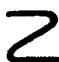
\includegraphics[keepaspectratio]{images/part001_587db9d1.jpg}}

\section{DIMENSION OF GRADED RINGS}

In this section, we denote by H a graded ring of type Z, with positive degrees, and by \((\mathrm{H}_{n})_{n\in\mathbf{Z}}\) its grading; thus we have \(H_{n}=\{0\}\) for n\textless0.

\subsection{Filtered ring associated with a graded ring}

For every \(n \in \mathbf{Z}\) , we set \(\mathrm{H}_{\geqslant n} = \sum_{i \geqslant n} \mathrm{H}_i\) . We have \(\mathrm{H} = \mathrm{H}_{\geqslant 0}\) ; the \(\mathrm{H}_{\geqslant n}\) are graded ideals of \(\mathrm{H}\) . Let S be the multiplicative subset \(1 + \mathrm{H}_{\geqslant 1}\) formed by the elements of H whose component of degree 0 is equal to 1, and consider the ring of fractions \(\mathrm{S}^{-1}\mathrm{H}\) . Identify H with a subring of its completion \(\hat{\mathrm{H}} = \prod_{n} \mathrm{H}_{n}\) (III, § 2, no. 12, example 1); since the elements of S are invertible in \(\hat{\mathrm{H}}\) (III, § 2, no. 13, lemma 3), \(\mathrm{S}^{-1}\mathrm{H}\) is identified with a subring of \(\hat{\mathrm{H}}\) containing H. For \(s \in \mathrm{S}\) and \(h \in \mathrm{H}_{\geqslant n}\) , the element \(s^{-1}h - h\) of \(\hat{\mathrm{H}}\) belongs to \(\prod_{i \geqslant n} \mathrm{H}_i\) ; consequently we have \(\mathrm{S}^{-1}\mathrm{H}_{\geqslant n} = (\mathrm{S}^{-1}\mathrm{H}) \cap \prod_{i \geqslant n} \mathrm{H}_i\) .

We deduce from this:

PROPOSITION 1. --- a) The ideals S \(^{-1}\) H \(_{≥n}\) form an exhaustive and separated filtration of the ring S \(^{-1}\) H.

\begin{enumerate}
\def\labelenumi{\alph{enumi})}
\setcounter{enumi}{1}
\tightlist
\item
  The canonical homomorphism from H to \(S^{-1}H\) induces for each n an isomorphism \(u_{n}\) of \(H_{n}\) onto \(S^{-1}H_{\geqslant n}/S^{-1}H_{\geqslant n+1}\) ; the \(u_{n}\) are the homogeneous components of an isomorphism of graded rings from H onto the graded ring associated with \(S^{-1}H\) , filtered by the \(S^{-1}H_{\geqslant n}\) .
\end{enumerate}

Remarks. --- 1) An element \(h/s\) of \(\mathrm{S}^{-1}\mathrm{H}\) with \(h\in\mathrm{H}, s\in\mathrm{S}\) , is invertible if and only if the component of degree 0 of \(h\) is invertible in \(\mathrm{H}_{0}\) . Consequently, if the ring \(\mathrm{H}_{0}\) is local, the ring \(\mathrm{S}^{-1}\mathrm{H}\) is local and the canonical injection \(\mathrm{H}_{0}\to\mathrm{S}^{-1}\mathrm{H}\) induces an isomorphism on the residue fields.

\begin{enumerate}
\def\labelenumi{\arabic{enumi})}
\setcounter{enumi}{1}
\tightlist
\item
  Suppose H is generated by \(H_{0}\) and \(H_{1}\) ; then for every n, we have \(H_{n+1} = H_{1}.H_{n}\) , hence \(H_{\geqslant n+1} = H_{1}.H_{\geqslant n}\) and \(S^{-1}H_{\geqslant n+1} = H_{1}.S^{-1}H_{\geqslant n}\) . Consequently, the filtration \((S^{-1}H_{\geqslant n})\) of \(S^{-1}H\) is the filtration \(S^{-1}H_{\geqslant 1}\) -adic.
\end{enumerate}

Examples. --- 1) * Let p be a graded prime ideal of C{[}X₀, \ldots, Xₙ{]} different from the ideal generated by the Xᵢ; let V be the algebraic subvariety of Pⁿ(C) defined by p and C the algebraic subvariety of Cⁿ⁺¹ defined by p. Then C is the cone over V, H = C{[}X₀, \ldots, Xₙ{]}/p is the affine algebra of C and S⁻¹H is the local ring of the cone C at its vertex. *

\begin{enumerate}
\def\labelenumi{\arabic{enumi})}
\setcounter{enumi}{1}
\tightlist
\item
  Let A be a local ring and a an ideal of A distinct from A. Then H = \(\bigoplus_{n} \mathfrak{a}^{n}/\mathfrak{a}^{n+1}\)
\end{enumerate}

is a graded ring such that \(H_{0} = A/\mathfrak{a}\) is local; it is generated by \(H_{0}\) and \(H_{1}\) . The ring \(S^{-1}H\) is therefore local and the filtration ( \(S^{-1}H_{\geq n}\) ) is the \(S^{-1}H_{\geq 1}\) -adic filtration. Note that in general the rings A and \(S^{-1}H\) are not isomorphic. * In particular, an algebraic variety is not in general locally isomorphic, in a neighborhood of a point, to its tangent cone at that point. *

\subsection{Dimension and chains of graded ideals}

In this issue, we will denote by dimgr(H) the supremum of the lengths of chains of graded prime ideals of H; likewise, if p is a graded prime ideal of H, we will denote by htgr(p) the supremum of the lengths of chains of graded prime ideals of H for which p is the largest element. If p is a graded prime ideal of H, we have \(p \cap S = \varnothing\); otherwise, indeed p would contain an element whose degree-0 component equals 1, hence would contain 1 since it is graded. The map \(p \mapsto S^{-1}p\) from the set of graded prime ideals of H to the set of prime ideals of \(S^{-1}H\) is therefore injective and increasing (II, § 2, no. 5, prop. 11); consequently, in view of § 1, no. 3, prop. 6 and the corollary to prop. 7, we have:

PROPOSITION 2. --- a) We have \(\dim \mathrm{gr}(\mathrm{H}) \leqslant \dim (\mathrm{S}^{-1}\mathrm{H}) \leqslant \dim (\mathrm{H})\) .

\begin{enumerate}
\def\labelenumi{\alph{enumi})}
\setcounter{enumi}{1}
\tightlist
\item
  For every graded prime ideal \(\mathfrak{p}\) from H, we have \(\operatorname{htgr}(\mathfrak{p}) \leqslant \operatorname{ht}(\mathrm{S}^{-1}\mathfrak{p}) = \operatorname{ht}(\mathfrak{p})\) .
\end{enumerate}

For every ideal a of H, denote \(a^{gr}\) the largest graded ideal contained in a; we have \(a^{gr} = \sum_{n} (a \cap H_n)\) .

Lemma 1. --- a) If p is a prime ideal of H, \(\mathfrak{p}^{\mathrm{gr}}\) is a prime ideal.

\begin{enumerate}
\def\labelenumi{\alph{enumi})}
\setcounter{enumi}{1}
\item
  Every maximal element of the set of graded ideals of H distinct from H is a maximal ideal of H that contains \(H_{\geq1}\) .
\item
  Every minimal prime ideal of H is graded.
\item
  This follows from III, § 1, no. 4, prop. 4.
\item
  Let m be a graded ideal of H distinct from H. Then we have
\end{enumerate}

\[
\mathfrak {m} \subset (\mathfrak {m} \cap \mathrm{H} _ {0}) + \mathrm{H} _ {\geqslant 1} \neq \mathrm{H}.
\]

If m is maximal, then we have \(m = m_{0} + H_{\geq 1}\) , where \(m_{0}\) is a maximal ideal of \(H_{0}\) , whence b).

\begin{enumerate}
\def\labelenumi{\alph{enumi})}
\setcounter{enumi}{2}
\tightlist
\item
  Let p be a minimal prime ideal of H. Since \(p^{gr}\) is prime by a) and contained in p, we have \(p = p^{gr}\) whence c).
\end{enumerate}

Lemma 2.---Let p and q be prime ideals of H such that q ⊂ p and q ≠ p. If q \(^{gr}\) = p \(^{gr}\) then q is graded, p is not, and ht(p/q) = 1.

Remark 1.--- Let us take up the notations of example 1 of no. 1. Lemma 2 implies that, if two irreducible subvarieties Y and Z of \(\mathbf{C}^{n+1}\) have the same projecting cone and if \(Z \subset Y\) and \(Z \neq Y\) , then Y is the projecting cone of Z, and Z has codimension 1 in Y. *

Replacing H by \(\mathrm{H} / \mathfrak{q}^{\mathrm{gr}}\) we reduce to the case where \(\mathfrak{q}^{\mathrm{gr}} = \{0\}\). Then H is integral (lemma 1, a)), \(\mathfrak{p}^{\mathrm{gr}} = 0\) , and the task is to prove that \(\operatorname{ht}(\mathfrak{p}) \leqslant 1: this will indeed imply that  \operatorname{ht}(\mathfrak{q}) = 0\) , hence that \(\mathfrak{q} = \{0\}\) . Since \(\mathfrak{p}^{\mathrm{gr}} = \{0\}\) , one has \(\mathfrak{p} \cap \mathrm{H}_n = \{0\}\) for every \(n\) , and \(\mathfrak{p}\) is disjoint from the multiplicative subset \(\mathrm{T} = \bigcup_{n} (\mathrm{H}_n - \{0\})\) . The ring \(\mathrm{H}_{\mathfrak{p}}\) is therefore isomorphic to a ring of fractions of \(\mathrm{T}^{-1}\mathrm{H}\) , and we therefore have

\[
\mathrm{ht} (\mathfrak {p}) = \dim (\mathrm{H} _ {\mathfrak {p}}) \leqslant \dim (\mathrm{T} ^ {- 1} \mathrm{H})
\]

(§ 1, no. 3, props. 6 and 7). But, by Lemma 4 of V, § 1, no. 8, T \(^{-1}\) H is a field or is isomorphic to a ring K{[}X, X \(^{-1}\) {]}, where K is a field; we therefore have dim(T \(^{-1}\) H) ≤ 1 and ht(p) ≤ 1, which is what we wanted to prove.

PROPOSITION 3. --- Let p be a prime ideal of H. If p ≠ p \(^{gr}\) , we have ht(p \(^{gr}\) ) = ht(p) - 1. By Lemma 1, a), the ideal p \(^{gr}\) is prime and contained in p, hence ht(p \(^{gr}\) ) ≤ ht(p) - 1. The proposition being trivial when ht(p \(^{gr}\) ) = +∞, we may assume ht(p \(^{gr}\) ) \textless{} + ∞. Let us prove the inequality ht(p) ≤ ht(p \(^{gr}\) ) + 1 by induction on ht(p \(^{gr}\) ). It suffices to prove that, for every prime ideal q contained in p and distinct from p, one has ht(q) ≤ ht(p \(^{gr}\) ). We distinguish two cases according as q \(^{gr}\) ≠ p \(^{gr}\) or that q \(^{gr}\) = p \(^{gr}\) . If q \(^{gr}\) ≠ p \(^{gr}\) , then we have ht(q \(^{gr}\) ) \textless{} ht(p \(^{gr}\) ); we have

\[
\mathrm{ht} (\mathfrak {q}) \leqslant \mathrm{ht} (\mathfrak {q} ^ {\mathrm{gr}}) + 1,
\]

by the induction hypothesis if q ≠ q \(^{gr}\) and trivially if q = q \(^{gr}\) ; consequently, we have ht(q) ≤ ht(q \(^{gr}\) ) + 1 ≤ ht(p \(^{gr}\) ), which is what we wanted to prove. If q \(^{gr}\) = p \(^{gr}\) , then we have q = q \(^{gr}\) by Lemma 2, hence ht(q) = ht(q \(^{gr}\) ) ≤ ht(p \(^{gr}\) ), whence again the desired conclusion.

THEOREM 1. --- Assume H is Noetherian.

\begin{enumerate}
\def\labelenumi{\alph{enumi})}
\item
  Every chain of graded prime ideals of H, saturated as a chain of graded prime ideals, is saturated as a chain of prime ideals.
\item
  For every graded prime ideal p of H, one has htgr(p) = ht(S \(^{-1}\) p) = ht(p).
\item
  We have \(\dim \mathrm{gr}(\mathbf{H}) = \dim (\mathbf{S}^{-1}\mathbf{H}) = \dim (\mathbf{H}).\)
\end{enumerate}

To prove \(a\) ), it suffices to show that, if \(\mathfrak{p}\) and \(\mathfrak{q}\) are two distinct graded prime ideals of H such that \(\mathfrak{q} \subset \mathfrak{p}\) and every graded prime ideal between \(\mathfrak{q}\) and \(\mathfrak{p}\) is equal to \(\mathfrak{p}\) or to \(\mathfrak{q}\) , then \(\mathrm{ht}(\mathfrak{p}/\mathfrak{q}) = 1\) . By dividing by \(\mathfrak{q}\) , one reduces to the case where \(\mathfrak{q} = \{0\}\) . It therefore remains to prove that, if H is integral, and if \(\mathfrak{p}\) is an ideal of H, minimal among the graded prime ideals \(\neq \{0\}\) , one has \(\mathrm{ht}(\mathfrak{p}) = 1\) . Now let \(a\) be a nonzero homogeneous element of \(\mathfrak{p}\) , and let r be a prime ideal of H such that \(a \in \mathfrak{r} \subset \mathfrak{p}\) and minimal for these properties (II, § 2, no. 6, lemma 2). Since \(\mathfrak{r}^{\mathrm{gr}}\) is prime (lemma 1, \(a\) ) and nonzero, we have \(\mathfrak{r}^{\mathrm{gr}} = \mathfrak{p}\) , hence \(\mathfrak{p} = \mathfrak{r}\) . Since H is integral and Noetherian, \(\mathfrak{p}\) has height 1 (§ 3, no. 1, prop. 1), whence \(a\) ).

Let us prove b). Let p be a graded prime ideal of H. We have

\[
\operatorname{htgr} (\mathfrak {p}) \leqslant \operatorname{ht} \left(\mathrm{S} ^ {- 1} \mathfrak {p}\right) \leqslant \operatorname{ht} (\mathfrak {p})
\]

(prop. 2); let us prove the inequality ht(p) ≤ htgr(p) by induction on htgr(p). If htgr(p) = 0, p is minimal among graded prime ideals, hence minimal (lemma 1, c)), and we have ht(p) = 0. Suppose that htgr(p) \textgreater{} 0 and let us prove the inequality ht(q) ≤ htgr(p) - 1 for every prime ideal q contained in p and distinct from p. Let us distinguish two cases. If q is graded, we conclude by the induction hypothesis. If q is not graded, then we have q \(^{gr}\) ≠ p, hence ht(q \(^{gr}\) ) ≤ htgr(q \(^{gr}\) ) by the induction hypothesis, whence ht(q) ≤ htgr(q \(^{gr}\) ) + 1 by prop. 3; it remains to prove the inequality htgr(q \(^{gr}\) ) ≤ htgr(p) - 2; but if we had htgr(q \(^{gr}\) ) = htgr(p) - 1, the chain q \(^{gr}\) ⊂ p would be saturated by a), which is not the case since q \(^{gr}\) ≠ q ≠ p.

Let us finally prove c). We have dimgr(H) ≤ dim(S⁻¹H) ≤ dim(H) (prop. 2), and it remains to prove dim(H) ≤ dimgr(H), or equivalently ht(p) ≤ dimgr(H) for every prime ideal p of H. Let p therefore be a prime ideal of H. If p is graded, we have ht(p) = htgr(p) ≤ dimgr(H). If p is not graded, we have ht(p) = htgr(p\(^{\mathrm{gr}}\)) + 1 by prop. 3; let m be a maximal graded ideal of H containing p\(^{\mathrm{gr}}\); by lemma 1, b), m is maximal, hence distinct from p\(^{\mathrm{gr}}\), and we have htgr(p\(^{\mathrm{gr}}\)) + 1 ≤ htgr(m) ≤ dimgr(H), whence again ht(p) ≤ dimgr(H). This completes the proof.

Remark 2. --- There exist non-Noetherian graded rings H such that dimgr(H) \textless{} dim(H) (p.~99, exercise 1).

\subsection{Dimension of graded modules}

In this number, we denote by M a graded H-module (of type Z).

Then \(\mathbf{S}^{-1}\mathbf{M}\) is an \(\mathbf{S}^{-1}\mathbf{H}\)-module, and if we set \(\mathbf{M}_{\geqslant n} = \bigoplus_{i\geqslant n}\mathbf{M}_i\) , we see as in

no. 1 that the sequence of sets \(S^{-1}M_{\geqslant n}\) is an exhaustive and separated filtration on

\(S^{-1}M\) and that the canonical map \(M \to S^{-1}M\) induces an isomorphism from M onto the graded module \(\oplus S^{-1}M_{\geqslant n}/S^{-1}M_{\geqslant n+1}\) .

Lemma 3. --- Suppose H is generated by \(\mathbf{H}_{0} \cup \mathbf{H}_{1}\) and M generated by \(\bigoplus_{i \leqslant n_{0}} \mathbf{M}_{i}\) for a suitable integer \(n_{0}\). Then the filtration \((\mathbf{S}^{-1}\mathbf{M}_{\geqslant n})\) of \(\mathbf{S}^{-1}\mathbf{M}\) is good for the ideal \(\mathbf{S}^{-1}\mathbf{H}_{\geqslant 1}\) of \(\mathbf{S}^{-1}\mathbf{H}\) .

We have, for \(n \geqslant n_0\) , \(\mathbf{M}_{\geqslant n+1} = \mathbf{H}_1 \cdot \mathbf{M}_{\geqslant n}\) , hence \(\mathbf{S}^{-1} \mathbf{M}_{\geqslant n+1} = \mathbf{H}_1 \cdot \mathbf{S}^{-1} \mathbf{M}_{\geqslant n} = \mathbf{S}^{-1} \mathbf{H}_{\geqslant 1} \cdot \mathbf{S}^{-1} \mathbf{M}_{\geqslant n}\) .

PROPOSITION 4. --- Suppose H is Noetherian and M is finitely generated. Then \(\dim_{\mathbf{H}}(\mathbf{M}) = \dim_{\mathbf{S}^{-1}\mathbf{H}}(\mathbf{S}^{-1}\mathbf{M})\) .

Let a be the annihilator of the H-module M; it is a graded ideal of H. Since M is a finitely generated H-module, the annihilator of the S \(^{-1}\) H-module S \(^{-1}\) M is the ideal S \(^{-1}\) a of S \(^{-1}\) H. We have dim \(_{H}\) (M) = dim(H/a) and dim \(_{S^{-1}H}\) (S \(^{-1}\) M) = dim(S \(^{-1}\) H/S \(^{-1}\) a). Prop. 4 then follows from th. 1, c) of no. 2 applied to the graded ring H/a.

Proposition 5. — Suppose \(\mathbf{H}_{0}\) is local and Artinian, \(\mathbf{H}\) is generated by \(\mathbf{H}_{0} \cup \mathbf{H}_{1}\) , \(\mathbf{H}_{1}\) is of finite type as a \(\mathbf{H}_{0}\) -module, and \(\mathbf{M}\) is nonzero and of finite type as an \(\mathbf{H}\) -module. Then \(\mathbf{M}_{n}\) is a nonzero finitely generated \(\mathbf{H}_{0}\) -module of finite length for each \(n\) , and there exists \(\mathbf{Q}(\mathbf{T}) \in \mathbf{Z}[\mathbf{T}, \mathbf{T}^{-1}]\) such that \(\mathbf{Q}(1) > 0\) and that one has in the ring \(\mathbf{Z}((\mathbf{T}))\)

\[
\sum_ {n \in \mathbf {Z}} \mathrm{long} _ {\mathrm{H} _ {0}} (\mathrm{M} _ {n}). \mathrm{T} ^ {n} = (1 - \mathrm{T}) ^ {- d}. \mathrm{Q} (\mathrm{T}),
\]

with \(d = \dim_{\mathbf{H}}(\mathbf{M})\).

The ring \(\mathbf{S}^{-1}\mathbf{H}\) is local and Noetherian (no. 1, remark 1), the \(\mathbf{S}^{-1}\mathbf{H}\) -module \(\mathbf{S}^{-1}\mathbf{M}\) is nonzero of finite type, and of dimension \(d = \dim_{\mathbf{H}}(\mathbf{M})\) (prop. 4). Moreover, \(\mathbf{S}^{-1}\mathbf{H}_{\geqslant 1}\) is a defining ideal of \(\mathbf{S}^{-1}\mathbf{H}\) (§ 3, no. 2, Lemma 2) and \(\mathbf{S}^{-1}\mathbf{M}_{\geqslant n}\) is a filtration \(\mathbf{S}^{-1}\mathbf{H}_{\geqslant 1}\) -good on \(\mathbf{S}^{-1}\mathbf{M}\) (Lemma 3). Finally, we have long \(_{\mathbf{S}^{-1}\mathbf{H}}\mathbf{S}^{-1}\mathbf{M}_{\geqslant n}/\mathbf{S}^{-1}\mathbf{M}_{\geqslant n+1} = \text{long}_{\mathbf{H}_0}(\mathbf{M}_n)\) for every \(n\). It therefore suffices to apply theorems 2 and 3 of § 4 (nos. 3 and 4).

Remark. --- Except for the determination of the integer d, prop. 5 follows directly from th. 1 of § 4, no. 2.

COROLLARY. --- Let A be a Noetherian local ring and q an ideal of definition of A. Then we have \(\dim(A) = \dim(\text{gr}_{\mathfrak{q}}(A))\) .

Applying prop. 5 to the case M = H = gr\_q(A), we obtain the relation

\[
\sum_ {n \geqslant 0} \mathrm{long} _ {\mathrm{A} / \mathfrak {q}} (\mathfrak {q} ^ {n} / \mathfrak {q} ^ {n + 1}). \mathrm{T} ^ {n} = (1 - \mathrm{T}) ^ {- d} \mathrm{Q} (\mathrm{T})
\]

with \(d = \dim(\mathrm{gr}_{\mathfrak{q}}(\mathbf{A}))\) and \(\mathbf{Q}(1) \neq 0\) . We have \(d = \dim(\mathbf{A})\) by th. 3 of § 4, no. 4, whence the corollary.

PROPOSITION 6. --- Suppose \(\mathbf{H}_{0}\) is local and Artinian, \(\mathbf{H}\) is of finite type as a \(\mathbf{H}_{0}\) -algebra and \(\mathbf{M}\) is of finite type as a \(\mathbf{H}\) -module.

\begin{enumerate}
\def\labelenumi{\alph{enumi})}
\item
  Let \(a_1, \ldots, a_n\) be elements of H, homogeneous of degrees \(> 0\) , and let \(\varphi\) be the homomorphism (of \(\mathbf{H}_0\) -algebras) from \(\mathbf{H}_0[\mathbf{X}_1, \ldots, \mathbf{X}_n]\) to H which sends \(\mathbf{X}_i\) to \(a_i\) for \(1 \leqslant i \leqslant n\) . The \(S^{-1}H\) -module \(S^{-1}M / \sum_{i=1}^{n}(a_i/1) \cdot S^{-1}M\) is of finite length if and only if \(\varphi_*(M)\) is a finitely generated module over \(\mathbf{H}_0[\mathbf{X}_1, \ldots, \mathbf{X}_n]\) .
\item
  There exists a family \((a_{1},...,a_{d})\) of elements of H, all homogeneous of the same degree \textgreater0, with \(d=\dim_{\mathrm{H}}(\mathbf{M})\) and such that \((a_{1}/1,...,a_{d}/1)\) is a maximal secant sequence for the \(S^{-1}H\) -module \(S^{-1}M\) . If moreover H is generated by \(H_{1}\) as \(H_{0}\) -algebra, and if the residue field of \(H_{0}\) is infinite, one may take the \(a_{i}\) of degree 1.
\item
  Set \(\mathbf{N} = \mathbf{M} / \sum_{i=1}^{n} a_i \mathbf{M}\) . We have \(\dim_{\mathrm{H}}(\mathbf{N}) = \dim_{\mathrm{S}^{-1}\mathrm{H}}(\mathrm{S}^{-1}\mathrm{N})\) by prop. 4. Consequently, the \(\mathrm{S}^{-1}\mathrm{H}\) -module \(\mathrm{S}^{-1}\mathrm{N}\) is of finite length if and only if the H-module N is of finite length, that is, if and only if N is a \(\mathrm{H}_0\) -module of finite type. If \(\varphi_*(\mathbf{M})\) is the module over \(\mathrm{H}_0[\mathrm{X}_1, ..., \mathrm{X}_n]\) deduced from M by the homomorphism \(\varphi : \mathrm{H}_0[\mathrm{X}_1, ..., \mathrm{X}_n] \to \mathbf{H}\) , one has \(\mathbf{N} = \varphi_*(\mathbf{M}) / \sum_{i=1}^{n} X_i \cdot \varphi_*(\mathbf{M})\) . Consequently (A, II, p.~171, cor. 3 and remark) \(\varphi_*(\mathbf{M})\) is a finitely generated module over \(\mathrm{H}_0[\mathrm{X}_1, ..., \mathrm{X}_n]\) if and only if N is a \(\mathrm{H}_0\) -module of finite type. This proves a).
\end{enumerate}

To prove b), we will first establish a lemma.

Lemma 4. --- Let \(b\) be an element of H, homogeneous of degree \(>0\), and not belonging to any of the minimal elements \(\mathfrak{p}\) of \(\operatorname{Supp}(\mathbf{M})\) such that \(\dim(\mathrm{H}/\mathfrak{p}) = \dim_{\mathrm{H}}(\mathbf{M})\). We then have \(\dim_{\mathrm{H}}(\mathbf{M}/b\mathbf{M}) = \dim_{\mathrm{H}}(\mathbf{M}) - 1\).

Set \(d = \dim_{\mathbf{H}}(\mathbf{M})\). By the definition of \(b\) , one has \(\dim_{\mathbf{H}}(\mathbf{M}/b\mathbf{M}) < d\). By prop. 4, we have

\[
\dim_ {\mathrm{H}} (\mathrm{M} / b \mathrm{M}) = \dim_ {\mathrm{S} ^ {- 1} \mathrm{H}} \left(\mathrm{S} ^ {- 1} \mathrm{M} / (b / 1). \mathrm{S} ^ {- 1} \mathrm{M}\right)
\]

and formula (8) of § 3, no. 2 yields the inequality

\[
\dim_ {\mathrm{S} ^ {- 1} \mathrm{H}} (\mathrm{S} ^ {- 1} \mathrm{M} / (b / 1). \mathrm{S} ^ {- 1} \mathrm{M}) \geqslant \dim_ {\mathrm{S} ^ {- 1} \mathrm{H}} (\mathrm{S} ^ {- 1} \mathrm{M}) - 1.
\]

Finally, we have

\[
\dim_ {S ^ {- 1} H} (S ^ {- 1} M) = \dim_ {H} (M) = d
\]

by prop. 4. We therefore have \(\dim_{\mathrm{H}}(\mathrm{M}/b\mathrm{M}) \geqslant d - 1\) , whence lemma 4.

Let us resume the proof of prop. 6, b). We may assume \(\dim_{\mathbf{H}}(\mathbf{M}) > 0\). Note that every minimal element of \(\operatorname{Supp}(\mathbf{M})\) is graded (apply Lemma 1 of No. 2 to the quotient of H by the annihilator of M). By Prop. 8 of III, § 1, No. 4, there therefore exists a homogeneous element \(b\) of H, of degree \(>0\), not belonging to any of the minimal elements \(\mathfrak{p}\) of \(\operatorname{Supp}(\mathbf{M})\) such that \(\dim(\mathrm{H}/\mathfrak{p}) = \dim_{\mathbf{H}}(\mathbf{M})\). By Lemma 4, we have \(\dim_{\mathbf{H}}(\mathbf{M}/b\mathbf{M}) = \dim_{\mathbf{H}}(\mathbf{M}) - 1\). Suppose moreover that H is generated by \(\mathrm{H}_{1}\) as \(\mathrm{H}_{0}\) -algebra and the residue field \(k\) of \(\mathrm{H}_{0}\) is infinite. For every minimal element \(\mathfrak{p}\) of \(\operatorname{Supp}(\mathbf{M})\) such that \(\dim(\mathrm{H}/\mathfrak{p}) = \dim_{\mathbf{H}}(\mathbf{M})\) , consider the vector subspace \(\mathrm{V}_{\mathfrak{p}} = (\mathfrak{p} \cap \mathrm{H}_{1}) \otimes_{\mathrm{H}_{0}} k\) of the \(k\)-vector space \(\mathrm{V} = \mathrm{H}_{1} \otimes_{\mathrm{H}_{0}} k\). If one had \(\mathrm{V}_{\mathfrak{p}} = \mathrm{V}\) , one would have \(\mathfrak{p} \cap \mathrm{H}_1 = \mathrm{H}_1\) (II, §3, no. 2, prop. 4), whence \(\mathrm{H}_1 \subset \mathfrak{p}\) and \(\dim_{\mathrm{H}}(\mathbf{M}) = \dim(\mathrm{H}/\mathfrak{p}) \leqslant \dim(\mathrm{H}/\mathrm{H}_{\geqslant 1}) = 0\) , which is not the case. Since \(k\) is assumed to be infinite, the union of the \(\mathrm{V}_{\mathfrak{p}}\) is distinct from V; if \(b \in \mathrm{H}_1\) is such that \(b \otimes 1\) belongs to none of the \(\mathrm{V}_{\mathfrak{p}}\) , one has \(\dim(\mathrm{M}/b\mathrm{M}) = \dim_{\mathrm{H}}(\mathrm{M}) - 1\) .

Proceeding by induction on \(d = \dim_{\mathbf{H}}(\mathbf{M})\) , one then constructs a sequence \((b_1, \ldots, b_d)\) of elements of H, with \(b_i\) homogeneous of degree \(n_i > 0\) and such that \(\mathbf{M} / \sum_{i=1}^{n} b_i \mathbf{M}\) is an H-module of finite length. If one assumes H is generated by \(\mathbf{H}_1\) as \(\mathbf{H}_0\) -algebra and the residue field of \(\mathbf{H}_0\) infinite, one may assume \(n_i = 1\) for \(i = 1, \ldots, d\). By prop. 4, we have \(\dim_{\mathbf{S}^{-1}\mathbf{H}}(\mathbf{S}^{-1}\mathbf{M}) = d\) and

\[
\dim_ {\mathrm{S} ^ {- 1} \mathrm{H}} (\mathrm{S} ^ {- 1} \mathrm{M} / \sum_ {i = 1} ^ {d} (b _ {i} / 1). \mathrm{S} ^ {- 1} \mathrm{M}) = 0.
\]

Then \((b_{1} / 1,\dots,b_{d} / 1)\) is a maximal secant sequence for the \(\mathbf{S}^{-1}\mathbf{H}\) -module \(\mathbf{S}^{-1}\mathbf{M}\) . Put \(a_{i} = b_{i}^{(n_{1}\dots n_{d}) / n_{i}}\) for \(1\leqslant i\leqslant d\) ; then the \(a_{i}\) are all of the same degree, and \((a_{1} / 1,\dots,a_{d} / 1)\) is a maximal secant sequence for \(\mathbf{S}^{-1}\mathbf{M}\) (§ 3, no. 2, Remark 3).

COROLLARY 1. --- Suppose that \(\mathbf{H}_0\) is a field and that \(\mathbf{H}\) is of finite type as an \(\mathbf{H}_0\) -algebra. Set \(n = \dim(\mathbf{H})\) . There exist homogeneous elements \(a_1, ..., a_n\) of \(\mathbf{H}\) all of the same degree \(>0\) , such that the \(\mathbf{H}_0\) -homomorphism \(\varphi: \mathbf{H}_0[\mathbf{X}_1, ..., \mathbf{X}_n] \to \mathbf{H}\) defined by \(\varphi(\mathbf{X}_i) = a_i\) , \(i = 1, ..., n\) , be injective and make \(\mathbf{H}\) a finite \(\mathbf{H}_0[\mathbf{X}_1, ..., \mathbf{X}_n]\)-algebra. If \(\mathbf{H}\) is generated by \(\mathbf{H}_1\) as \(\mathbf{H}_0\) -algebra and if \(\mathbf{H}_0\) is infinite, one may assume the \(a_i\) of degree 1.

There exists, by prop. 6, a \(\mathbf{H}_0\) -homomorphism \(\varphi\) of the indicated form that makes H a \(\mathbf{H}_0[\mathbf{X}_1, \ldots, \mathbf{X}_n]\) -finite algebra. By th. 1 of § 2, no. 3, we then have

\[
\dim \left(\mathrm{H} _ {0} \left[ \mathrm{X} _ {1}, \dots , \mathrm{X} _ {n} \right] / (\operatorname{Ker} \varphi)\right) = \dim (\mathrm{H});
\]

since we have

\[
\dim (\mathrm{H}) = n = \dim \left(\mathrm{H} _ {0} \left[ \mathrm{X} _ {1}, \dots , \mathrm{X} _ {n} \right]\right),
\]

and that \(\mathrm{H}_0[\mathrm{X}_1, \dots, \mathrm{X}_n]\) is an integral domain, this implies \(\operatorname{Ker} \varphi = \{0\}\) .

Note. --- Let \((h_{1}, \ldots, h_{r})\) be a finite generating system of the \(H_{0}\) -vector space \(H_{1}\) . For \(\lambda = (\lambda_{1}, \ldots, \lambda_{r}) \in H_{0}^{r}\) , set \(h_{\lambda} = \lambda_{1} h_{1} + \cdots + \lambda_{r} h_{r}\). The proofs of Prop. 6 and Cor. 1 yield the following result: the set of elements \((\lambda_{1}, \ldots, \lambda_{n})\) of \((\mathrm{H}_{0}^{r})^{n}\) such that the elements \(a_{i} = h_{\lambda_{i}} \in H_{1}\) satisfy the conclusion of Cor. 1, contains the complement of the union of a finite number of vector subspaces of \((\mathrm{H}_{0}^{r})^{n}\) distinct from the entire space.

COROLLARY 2. --- Let A be a Noetherian local ring and \(n\in\mathbb{N}\). For one to have \(\dim(\mathbf{A})\geqslant n\) it is necessary and sufficient that for every integer \(r\geqslant0\) , one has

\[
\left[ \mathfrak {m} _ {\mathrm{A}} ^ {r} / \mathfrak {m} _ {\mathrm{A}} ^ {r + 1}: \kappa_ {\mathrm{A}} \right] \geqslant \binom {n + r - 1} {n - 1}, \quad \left(\text { resp.   long } _ {\mathrm{A}} (\mathrm{A} / \mathfrak {m} _ {\mathrm{A}} ^ {r + 1}) \geqslant \binom {n + r} {n}\right);
\]

We have equality for every r if and only if A is regular of dimension n.

The condition is sufficient (§ 4, no. 4, th. 3 and § 5, no. 2, th. 1). Let us show that it is necessary. Consider the graded ring gr(A) = gr \(_{m_A}\) (A); let k be an infinite extension of the field κ \(_A\) , and set H = k ⊗ κ \(_A\) gr(A). The ring H has dimension ≥ n (prop. 5 and its corollary); hence, from cor. 1, we deduce the existence of an injective graded homomorphism of graded k-algebras φ : H \(_0\) {[}X \(_1\) , \ldots, X \(_n\) {]} → H. Consequently, for every integer r ≥ 0,

\[
\left[ \mathrm{gr} _ {r} (\mathrm{A}): \kappa_ {\mathrm{A}} \right] = \left[ \mathrm{H} _ {r}: \mathrm{H} _ {0} \right] \geqslant \binom {n + r - 1} {n - 1},
\]

and the equality for every \(r\) implies the bijectivity of \(\varphi\) , hence the regularity of A ( \(\S\) 5, no. 2, th. 1).

The equalities

\[
\mathrm{long} _ {\mathbf {A}} (\mathrm{A} / \mathfrak {m} _ {\mathbf {A}} ^ {r + 1}) = \sum_ {i = 0} ^ {r} \left[ \mathrm{gr} _ {i} (\mathbf {A}): \kappa_ {\mathbf {A}} \right]
\]

and

\[
\binom {n + r} {n} = \sum_ {i = 0} ^ {r} \binom {n + i - 1} {n - 1}
\]

then imply the analogous assertions for the function \(r \mapsto \text{long}_{\mathbf{A}}(\mathbf{A}/m_{\mathbf{A}}^{r+1})\) .

\subsection{Semicontinuity of dimension}

Lemma 5.--- Let A be a ring, r its radical, \(\mathbf{R} = \bigoplus_{i \in \mathbf{Z}} \mathbf{R}_i\) a graded A-algebra, \(\mathbf{M} = \bigoplus_{i \in \mathbf{Z}} \mathbf{M}_i\) a graded R-module. We assume that each \(\mathbf{M}_i\) is an A-module of finite type

and that M/rM is a finitely generated R/rR-module. Then M is a finitely generated R-module. Let \(m_{1}, \ldots, m_{n}\) be homogeneous elements of M, whose images in M/rM generate the R/rR-module M/rM. Let N be the (graded) sub-R-module of M generated by \(\{m_{1}, \ldots, m_{n}\}\) . For every \(i \in \mathbf{Z}\) , one has \(M_{i} = N_{i} + rM_{i}\) , hence \(M_{i} = N_{i}\) (II, §3, no. 2, prop. 4); consequently, we have M = N.

Lemma 6. --- Let \(\rho: \mathbf{B} \to \mathbf{C}\) be a ring homomorphism and S a multiplicative subset of B. Suppose that C is a finitely generated B-algebra, and that \(\mathbf{S}^{-1}\mathbf{C}\) is a finite \(\mathbf{S}^{-1}\mathbf{B}\)-algebra. There then exists \(f \in \mathbf{S}\) such that \(\mathbf{C}_f\) is a finite \(\mathbf{B}_f\)-algebra.

Let X be a finite generating set of the B-algebra C. For every \(x \in X\), the image of x in \(S^{-1}C\) is integral over \(S^{-1}B\), and there consequently exist an integer \(n(x) \geqslant 0\), elements \(b_{1}(x), \ldots, b_{n(x)}(x) \in B\), and an element \(f(x) \in S\) such that

\[
f (x) x ^ {n (x)} + b _ {1} (x) x ^ {n (x) - 1} + \dots + b _ {n (x)} = 0.
\]

Let \(f = \prod_{x \in X} f(x)\) ; the image of every element \(x\) of \(X\) in \(C_f\) is integral over \(B_f\) , hence \(C_f\) is a finite \(B_f\)-algebra (V, § 1, no. 1, prop. 4).

PROPOSITION 7. — Suppose that H is an \(H_{0}\)-algebra of finite type. Then the function \(\mathfrak{p} \mapsto \dim(\mathrm{H} \otimes_{\mathrm{H}_{0}} \kappa(\mathfrak{p}))\) is upper semicontinuous on \(\operatorname{Spec}(\mathrm{H}_{0})\) .

Since H is finitely generated as an \(H_{0}\)-algebra, each \(H_{i}\) is a finitely generated \(H_{0}\)-module (III, § 1, no. 2, corollary to prop. 1), and H is generated as an \(H_{0}\)-algebra by \(H_{0} \oplus H_{1} \oplus \cdots \oplus H_{r}\) for a suitable integer \(r \geqslant 0\). Let \(\mathfrak{p} \in \operatorname{Spec}(H_{0})\) and set \(\dim(H \otimes_{H_{0}} \kappa(\mathfrak{p})) = n \geqslant 0\). By Corollary 1 to Prop. 6, there exist elements \(a_{1}, ..., a_{n}\) of H, all homogeneous of the same degree \(d > 0\), such that the \(\kappa(\mathfrak{p})\)-homomorphism \(\overline{\varphi}: \kappa(\mathfrak{p})[X_{1}, ..., X_{n}] \to H \otimes_{H_{0}} \kappa(\mathfrak{p})\) which maps \(X_{i}\) to \(a_{i} \otimes 1\) for \(1 \leqslant i \leqslant n\), makes \(H \otimes_{H_{0}} \kappa(\mathfrak{p})\) a finite \(\kappa(\mathfrak{p})[X_{1}, ..., X_{n}]\)-algebra. Let \(\varphi\) be the \(H_{0}\)-homomorphism from \(H_{0}[X_{1}, ..., X_{n}] = R\) to H which maps \(X_{i}\) to \(a_{i}\) for \(1 \leqslant i \leqslant n\). If one sets, for every \(m \in \mathbf{Z}\), \(H_{m}' = \sum_{(m-1)d < i \leqslant md} H_{i}\), one obtains a grading of type \(\mathbf{Z}\) on H, compatible with the R-module structure given by \(\varphi\). Each \(H_{m}'\) is of finite type over \(H_{0}\). By Lemma 5, \(H_{\mathfrak{p}}\) is a finitely generated \(R_{\mathfrak{p}}\)-module. By Lemma 6, there therefore exists \(f \in H_{0} - \mathfrak{p}\) such that \(H_{f}\) is an \(R_{f}\)-module of finite type. For every \(\mathfrak{q} \in \operatorname{Spec}(H_{0})_{f}\), \(H \otimes_{H_{0}} \kappa(\mathfrak{q})\) is a finite \(\kappa(\mathfrak{q})[X_{1}, ..., X_{n}]\)-algebra, hence \(\dim(H \otimes_{H_{0}} \kappa(\mathfrak{q})) \leqslant n\) (\S 2, n° 3, th. 1), which completes the proof.

Remarks. --- 1) * In algebraic geometry, prop. 7 implies that the dimension of the fibers of a projective morphism of algebraic varieties is upper semi-continuous. *

\begin{enumerate}
\def\labelenumi{\arabic{enumi})}
\setcounter{enumi}{1}
\tightlist
\item
  We will see later that if \(\rho:A\to B\) is a ring homomorphism that makes \(B\) a \(A\) -algebra of finite type, the function \(\mathfrak{q}\mapsto\dim_{\mathfrak{q}}(B\otimes_{A}\kappa(\rho^{-1}(q)))\) is upper semicontinuous on \(\operatorname{Spec}(B)\) (cf. p. 101, exerc. 10).
\end{enumerate}

\subsection{Graded regular algebras}

In this issue, we assume that \(H_{0}\) is a field and that H is an \(H_{0}\)-algebra of finite type.

One sets \(H_{+} = H_{\geqslant 1}\) ; it is a maximal ideal of H. The ring \(S^{-1}H\) is identified with the local ring \(H_{H_{+}}\) of H at the ideal \(H_{+}\) ; its maximal ideal is \((\mathrm{H}_{+})_{\mathrm{H}_{+}} = \mathrm{S}^{-1}\mathrm{H}_{+}\) , its residue field is identified with \(H_{0}\) .

PROPOSITION 8. --- a) We have \(\dim(\mathbf{H}) \leqslant [\mathbf{H}_{+}/\mathbf{H}_{+}^{2}:\mathbf{H}_{0}]\) .

\begin{enumerate}
\def\labelenumi{\alph{enumi})}
\setcounter{enumi}{1}
\tightlist
\item
  The following conditions are equivalent:
\end{enumerate}

\begin{enumerate}
\def\labelenumi{(\roman{enumi})}
\item
  \(\dim (\mathrm{H}) = [\mathrm{H}_{+} / \mathrm{H}_{+}^{2}:\mathrm{H}_{0}]\) ;
\item
  the Noetherian local ring \(\mathbf{S}^{-1}\mathbf{H}\) is regular ;
\item
  H is generated as \(H_{0}\) -algebra by a family of homogeneous elements of degrees \textgreater{} 0, algebraically independent over \(H_{0}\) .
\end{enumerate}

\begin{enumerate}
\def\labelenumi{\alph{enumi})}
\setcounter{enumi}{2}
\tightlist
\item
  Suppose the conditions of b) are satisfied, and let \(a_{1}, \ldots, a_{n} \in \mathbf{H}\) be homogeneous elements of degrees \textgreater{} 0. The following conditions are equivalent:
\end{enumerate}

\begin{enumerate}
\def\labelenumi{(\roman{enumi})}
\item
  the classes of \(a_{i}\) form a basis of the \(\mathbf{H}_{0}\) -vector space \(\mathbf{H}_{+}/\mathbf{H}_{+}^{2}\) ;
\item
  the \(a_{i}/1\) form a coordinate system of the regular Noetherian local ring \(\mathbf{S}^{-1}\mathbf{H}\) ;
\item
  the \(a_{i}\) are algebraically independent over \(\mathbf{H}_{0}\) and generate \(\mathbf{H}\) as \(\mathbf{H}_{0}\) -algebra.
\end{enumerate}

We have \(\dim(\mathbf{H})=\dim(\mathbf{S}^{-1}\mathbf{H})\) (no. 2, th. 1), and \([\mathbf{H}_{+}/\mathbf{H}_{+}^{2}:\mathbf{H}_{0}]=[(\mathbf{S}^{-1}\mathbf{H}_{+})/(\mathbf{S}^{-1}\mathbf{H}_{+})^{2}:\mathbf{H}_{0}]\) (II, § 3, no. 3, prop. 9); according to § 5, no. 1, this implies \(a\) ) and the equivalences (i) \(\Leftrightarrow\) (ii) in \(b\) ) and \(c\) ). The two implications (iii) \(\Rightarrow\) (i) in \(b\) ) and \(c\) ) are trivial. Let us prove the implications (i) \(\Rightarrow\) (iii). Suppose therefore that we have \(\dim(\mathbf{H})=[\mathbf{H}_{+}/\mathbf{H}_{+}^{2}:\mathbf{H}_{0}]\) and let \(a_{1},\ldots,a_{n}\) be homogeneous elements of H, of degrees \(>0\) , whose classes form a basis of \(\mathbf{H}_{+}/\mathbf{H}_{+}^{2}\) ; consider the homomorphism of graded algebras \(\varphi:\mathrm{H}_{0}[\mathrm{X}_{1},\ldots,\mathrm{X}_{n}]\to\mathrm{H}\) which sends \(\mathrm{X}_{i}\) onto \(a_{i}\) . The ideal \(\mathrm{H}_{+}\) of H is generated by the \(a_{i}\) (A, II, p.~171, cor. 2 and remark); consequently the homomorphism \(\varphi\) is surjective (III, § 1, no. 2, prop. 1). But we have

\[
\dim \left(\mathrm{H} _ {0} \left[ \mathrm{X} _ {1}, \dots , \mathrm{X} _ {n} \right]\right) = n = \dim (\mathrm{H}) = \dim \left(\mathrm{H} _ {0} \left[ \mathrm{X} _ {1}, \dots , \mathrm{X} _ {n} \right] / (\operatorname{Ker} \varphi)\right)
\]

(§ 2, no. 4, cor. 1 of th. 3), hence Ker φ = 0 since H₀{[}X₁, \ldots, Xₙ{]} is an integral domain. This implies assertions (iii).

Under the hypotheses of \(b\) ), one says that H is a regular \(\mathrm{H}_{0}\) -graded algebra, or a \(\mathrm{H}_{0}\) -graded polynomial algebra. Under the hypotheses of \(c\) ), we say that the \(a_{i}\) form a graded coordinate system of H.

Remarks. --- 1) With the notation of \(c\) ), let \(d_{i}\) be the degree of \(a_{i}\) ( \(1 \leqslant i \leqslant n\) ). Then the Poincaré series \(\mathbf{P}_{\mathrm{H}} = \sum_{n \in \mathbf{Z}} [\mathrm{H}_{n} : \mathrm{H}_{0}] \cdot \mathrm{T}^{n}\) is equal to \(\prod_{i} (1 - \mathrm{T}^{d_{i}})^{-1}\) (§4, no. 2, example 1). Consequently, if H is a \(\mathrm{H}_{0}\) -graded polynomial algebra, we have

\[
\mathrm{P} _ {\mathrm{H}} = \prod_ {n} (1 - \mathrm{T} ^ {n}) ^ {- \delta (n)}, \quad \text { with } \quad \delta (n) = \left[ (\mathrm{H} _ {+} / \mathrm{H} _ {+} ^ {2}) _ {n}: \mathrm{H} _ {0} \right].
\]

\begin{enumerate}
\def\labelenumi{\arabic{enumi})}
\setcounter{enumi}{1}
\tightlist
\item
  Conversely, the fact that there exist integers \(d_{i}>0\) such that \(\mathbf{P}_{\mathbf{H}}=\prod_{i}(1-\mathbf{T}^{d_{i}})^{-1}\) does not imply that H is a graded polynomial algebra; for example, if H is generated by an element X of degree 1 and an element Y of degree 2, subject only to the relation \(\mathbf{X}^{2}=0\) , one has \(\mathbf{P}_{\mathbf{H}}=(1-\mathbf{T})^{-1}\) .
\end{enumerate}

\section{MULTIPLICITIES}

Throughout this paragraph, let A denote a Noetherian ring.

\subsection{Multiplicity of a module with respect to an ideal}

Let M be a finitely generated A-module and q an ideal of A contained in the radical of A such that M/qM has finite length. Suppose M is not reduced to 0, and set \(d = \dim_{\mathbf{A}}(\mathbf{M})\). By § 4, no. 3, corollary of Th. 2 and no. 4, Remark 2, there exists a unique integer \(e_{\mathfrak{q}}(\mathbf{M}) > 0\) such that, for every integer \(n \geqslant 1\)

\[
\operatorname{long} _ {\mathbf {A}} (\mathrm{M} / \mathfrak {q} ^ {n + 1} \mathrm{M}) = e _ {\mathfrak {q}} (\mathrm{M}) \frac {n ^ {d}}{d !} + \beta_ {n} n ^ {d - 1}
\]

where \(\beta_{n}\) tends to a limit as \(n\) increases indefinitely.

DEFINITION 1. --- The integer \(e_{\mathfrak{q}}(\mathbf{M})\) is called the multiplicity of the A-module \(\mathbf{M}\) relative to the ideal q.

It is also denoted \(e_{\mathfrak{q}}^{\mathbf{A}}(\mathbf{M})\) when one wishes to mention the ring A. When A is local with maximal ideal m, one writes \(e(\mathbf{M})\) or \(e^{\mathbf{A}}(\mathbf{M})\) for \(e_{\mathfrak{m}}(\mathbf{M})\) or \(e_{\mathfrak{m}}^{\mathbf{A}}(\mathbf{M})\) .

Remarks. --- 1) If q' is an ideal of A contained in the radical of A and containing q, then \(e_{\mathfrak{q}'}(\mathbf{M}) \leqslant e_{\mathfrak{q}}(\mathbf{M})\) and, if the \(q'\)-adic filtration of M is q-good, we have \(e_{\mathfrak{q}'}(\mathbf{M}) = e_{\mathfrak{q}}(\mathbf{M})\) (§ 4, no. 3, th. 2).

\begin{enumerate}
\def\labelenumi{\arabic{enumi})}
\setcounter{enumi}{1}
\item
  If M is of finite length, we have \(e_{\mathfrak{q}}(\mathbf{M}) = \mathrm{long}_{\mathbf{A}}(\mathbf{M})\) (§ 4, no. 3, remark 3).
\item
  If \(d > 0\) , one has
\end{enumerate}

\[
\operatorname{long} _ {\mathrm{A} / \mathfrak {q}} (\mathfrak {q} ^ {n} \mathrm{M} / \mathfrak {q} ^ {n + 1} \mathrm{M}) = e _ {\mathfrak {q}} (\mathrm{M}) \frac {n ^ {d - 1}}{(d - 1) !} + \alpha_ {n} n ^ {d - 2}
\]

where \(\alpha_{n}\) tends to a limit as \(n\) increases indefinitely (§ 4, no. 3, corollary to th. 2).

\begin{enumerate}
\def\labelenumi{\arabic{enumi})}
\setcounter{enumi}{3}
\tightlist
\item
  One can reduce the computation of multiplicities to the case where A is local, since, by § 4, no. 4, corollary to th. 3, we have
\end{enumerate}

\[
e _ {\mathrm{q}} (\mathbf {M}) = \sum e _ {\mathrm{q} _ {\mathrm{m}}} (\mathbf {M} _ {\mathrm{m}})
\]

where the summation is extended over the maximal ideals m of A such that

\[
\mathfrak {m} \in \operatorname{Supp} (\mathbf {M}) \cap \mathrm{V} (\mathfrak {q}) \quad \text { and } \quad \dim_ {\mathrm{A} _ {\mathfrak {m}}} (\mathrm{M} _ {\mathfrak {m}}) = d  .
\]

It follows from Remarks 2 and 3 that \(e_{\mathfrak{q}}(\mathbf{M})\) depends only on the graded A/q-module \(\mathrm{gr}_{\mathfrak{q}}(\mathbf{M})\). Consequently:

PROPOSITION 1.--- Let \(\hat{\mathbf{A}}\) and \(\hat{\mathbf{M}}\) be the completions of \(\mathbf{A}\) and \(\mathbf{M}\) for their q-adic topologies; then \(e_{\mathfrak{q}}^{\mathbf{A}}(\mathbf{M}) = e_{\mathfrak{q}\hat{\mathbf{A}}}^{\hat{\mathbf{A}}}(\hat{\mathbf{M}})\) .

PROPOSITION 2. --- Suppose A is regular local (§ 5, no. 1, def. 1); then e(A) = 1.

This follows from th. 1 of § 5, no. 2.

Remark 5. --- One can have \(e(A) = 1\) without A being regular (p.~104, exerc. 5). In fact, a Noetherian local ring A is regular if and only if \(\hat{A}\) is an integral domain and if one has \(e(A) = 1\) (p.~108, exerc. 24).

Example. --- By definition, we have \(e_{\mathfrak{q}^{r}}(\mathbf{M}) = r^{d}e_{\mathfrak{q}}(\mathbf{M})\) where \(d = \dim_{\mathbf{A}}(\mathbf{M})\) . Consequently, if A is regular local, we have \(e_{\mathfrak{m}_{\mathbf{A}}^{r}}(\mathbf{A}) = r^{d}\) . For example, if A is a discrete valuation ring, we have \(e_{\mathfrak{q}}(\mathbf{A}) = \text{long}(\mathbf{A}/\mathfrak{q})\) .

Let q be an ideal of A contained in the radical of A, and let \(\mathcal{C}(\mathfrak{q})\) be the set of classes of finitely generated A-modules M such that \(M/qM\) has finite length. For every \(d \in \mathbf{N}\), denote by \(\mathcal{C}(\mathfrak{q})_{\leq d}\) the part of \(\mathcal{C}(\mathfrak{q})\) consisting of the classes of A-modules of dimension \(\leqslant d\). One defines a map \(e_{\mathfrak{q},d}: \mathcal{C}(\mathfrak{q})_{\leq d} \to \mathbf{Z}\) by \(e_{\mathfrak{q},d}(\mathbf{M}) = e_{\mathfrak{q}}(\mathbf{M})\) if \(\dim(\mathbf{M}) = d\), and \(e_{\mathfrak{q},d}(\mathbf{M}) = 0\) otherwise. This map is additive by prop. 5 of § 4, no. 3; from it one deduces (A, VIII, § 10, no. 2) a homomorphism, still denoted \(e_{\mathfrak{q},d}\), of the Grothendieck group \(K(\mathcal{C}(\mathfrak{q})_{\leq d})\) into \(\mathbf{Z}\), which vanishes on \(K(\mathcal{C}(\mathfrak{q})_{\leq d-1})\). Reasoning as in § 1, no. 5, we deduce:

PROPOSITION 3. — Let \(\mathbf{M}\) be a finitely generated A-module, of dimension \(d \geqslant 0\). Let \(\Phi\) be the set of minimal elements \(\mathfrak{p}\) of \(\operatorname{Supp}(\mathbf{M})\) such that \(\dim(\mathbf{A}/\mathfrak{p}) = d\). Let \(\mathfrak{q}\) be an ideal of A, contained in the radical of A, and such that \(\mathbf{M}/\mathfrak{q}\mathbf{M}\) is of finite length. We have

\[
e _ {\mathfrak {q}} (\mathrm{M}) = \sum_ {\mathfrak {p} \in \Phi} \operatorname{long} _ {\mathrm{A} _ {\mathfrak {p}}} (\mathrm{M} _ {\mathfrak {p}}) \cdot e _ {\mathfrak {q}} (\mathrm{A} / \mathfrak {p}).
\]

COROLLARY. — Suppose A is semi-local and let q be an ideal of definition of A.

\begin{enumerate}
\def\labelenumi{\alph{enumi})}
\item
  We have \(e_{\mathfrak{q}}(\mathbf{A}) = \sum_{\mathfrak{p}} e_{\mathfrak{q}}(\mathbf{A}/\mathfrak{p})\) , where \(\mathfrak{p}\) ranges over the set of minimal prime ideals of \(\mathbf{A}\) such that \(\dim(\mathbf{A}/\mathfrak{p}) = \dim(\mathbf{A})\) .
\item
  Suppose A is integral and let M be a finitely generated A-module such that \(\dim_{\mathbf{A}}(\mathbf{M}) = \dim(\mathbf{A})\) . Then one has \(e_{\mathfrak{q}}(\mathbf{M}) = \operatorname{rg}(\mathbf{M}) \cdot e_{\mathfrak{q}}(\mathbf{A})\) .
\end{enumerate}

\subsection{Multiplicities and flat extensions}

PROPOSITION 4. — Let \(\rho: A \to B\) be a local homomorphism of Noetherian local rings, and let \(N\) be a \(B\) -module, flat over \(A\) , and such that \(N \otimes_A \kappa_A\) is a \(B\) -module of finite length. If \(M\) is a nonzero finitely generated \(A\) -module and let q be an ideal of \(A\) distinct from \(A\) and such that \(M/qM\) is of finite length, then \((M \otimes_A N)/(qB)(M \otimes_A N)\) is a nonzero finitely generated \(B\) -module of finite length, and we have

\[
e _ {\mathrm{qB}} ^ {\mathrm{B}} (\mathbf {M} \otimes_ {\mathrm{A}} \mathbf {N}) = \operatorname{long} _ {\mathrm{B}} (\mathbf {N} \otimes_ {\mathrm{A}} \kappa_ {\mathrm{A}}). e _ {\mathrm{q}} ^ {\mathrm{A}} (\mathbf {M}).
\]

Let L be an A-module of finite length r. Then L possesses a Jordan-Hölder sequence of length r, with quotients isomorphic to \(\kappa_{A}\) ; since N is flat over A, the B-module \(L \otimes_{A} N\) possesses a composition sequence of length r, with quotients isomorphic to \(N \otimes_{A} \kappa_{A}\) , hence is of length \(r \cdot \operatorname{long}_{\mathbf{B}}(\mathbf{N} \otimes_{\mathbf{A}} \kappa_{\mathbf{A}})\). Since the B-module \((\mathbf{M} \otimes_{\mathbf{A}} \mathbf{N})/(\mathbf{q}\mathbf{B})^{n}(\mathbf{M} \otimes_{\mathbf{A}} \mathbf{N})\) is isomorphic to \((\mathbf{M}/\mathbf{q}^{n}\mathbf{M}) \otimes_{\mathbf{A}} \mathbf{N}\) for every \(n \in \mathbf{N}\), the proposition follows from the definition of multiplicities.

COROLLARY. — Suppose that B is flat over A and that \(\rho(\mathfrak{m}_{\mathbf{A}})\) B = \(\mathfrak{m}_{\mathbf{B}}\) . Then

\[
e _ {\mathbf {q B}} ^ {\mathbf {B}} (\mathbf {M} \otimes_ {\mathbf {A}} \mathbf {B}) = e _ {\mathbf {q}} ^ {\mathbf {A}} (\mathbf {M}).
\]

This applies in particular when B is the completion * or the henselization * of A with respect to an ideal distinct from A, * or an inflation of A, for example a strict henselization of A. *

Example. — * Let X be a complex algebraic variety, \(\mathcal{O}_{X,x}\) the local ring of X at a rational point \(x\) , \(X^{an}\) the analytic space associated with X; denote again by \(x\) the point of \(X^{an}\) corresponding to \(x\) , and let \(\mathcal{O}_{X^{an},x}\) be the local ring of \(X^{an}\) at \(x\) . Then \(e(\mathcal{O}_{X^{an},x}) = e(\mathcal{O}_{X,x})\) . *

\subsection{Multiplicities and finite extensions}

PROPOSITION 5. — Suppose A is semi-local and let \(\rho: A \to B\) be a ring homomorphism making B into a finitely generated A-module. Let N be a nonzero finitely generated B-module and let q be an ideal of A contained in the radical of A, and such that N/qN is of finite length. Among the maximal ideals of B (finite in number, by IV, § 2, no. 5, cor. 3 to prop. 9), denote by \(\mathfrak{m}_1, \ldots, \mathfrak{m}_r\) those for which we have \(\dim_{\mathrm{B}_{\mathfrak{m}_i}} (\mathrm{N}_{\mathfrak{m}_i}) = \dim_{\mathrm{B}} (\mathrm{N})\) . Put \(\mathbf{B}_i = \mathbf{B}_{\mathfrak{m}_i}\) and \(\mathfrak{q}_i = \mathfrak{q}\mathbf{B}_i\) for \(1 \leqslant i \leqslant r\) . Then we have the equalities

\[
\dim_ {A} (N) = \dim_ {B} (N),
\]

\[
e _ {\mathfrak {q} \mathrm{B}} ^ {\mathbf {B}} (\mathbf {N}) = \sum_ {i = 1} ^ {r} e _ {\mathfrak {q} _ {i}} ^ {\mathbf {B} _ {i}} (\mathbf {N} _ {\mathfrak {m} _ {i}}),
\]

\[
e _ {\mathfrak {q}} ^ {\mathrm{A}} (\mathrm{N}) = \sum_ {i = 1} ^ {r} \left[ \mathrm{B} / \mathfrak {m} _ {i}: \mathrm{A} / \rho^ {- 1} (\mathfrak {m} _ {i}) \right] e _ {\mathfrak {q} _ {i}} ^ {\mathrm{B} _ {i}} (\mathrm{N} _ {\mathfrak {m} _ {i}}).
\]

The first equality follows from § 2, no. 3, th. 1, c); the second follows from remark 4 of no. 1 (note that m \(_{i}\) belongs to V(qB) for \(1 \leqslant i \leqslant r\) since \(\rho^{-1}(m_{i}) \supset q\) by V, § 2, no. 1, prop. 1). Let us prove the third equality. Let E be a B-module of finite length; we have

\[
\operatorname{long} _ {\mathbf {A}} (\mathbf {E}) = \sum_ {m} \left[ \mathrm{B} / m: \mathrm{A} / \rho^ {- 1} (m) \right]. \operatorname{long} _ {\mathrm{B} _ {m}} \left(\mathrm{E} _ {m}\right),
\]

m ranging over the set of maximal ideals of B ; this is indeed evident when E is one of the B/m, and the general case follows from this, since E possesses a composition sequence whose quotients are isomorphic to B/m. Applying this formula to the B-modules N/q \(^{n+1}\) N, we deduce the desired equality by definition of multiplicities.

COROLLARY. — If \(\left[\mathrm{B}/\mathfrak{m}_{i}:\mathrm{A}/\rho^{-1}(\mathfrak{m}_{i})\right]=1\) for all i, we have \(e_{\mathfrak{q}}^{\mathrm{A}}(\mathrm{N})=e_{\mathfrak{q}\mathrm{B}}^{\mathrm{B}}(\mathrm{N})\) .

Lemma 1. — Let \(\rho: A \to B\) be a ring homomorphism, and let \(\mathfrak{p}\) be a prime ideal of A. Consider the following two properties:

\begin{enumerate}
\def\labelenumi{(\roman{enumi})}
\item
  the canonical homomorphism \(\tilde{\rho}\) from \(\mathbf{A}_{\mathfrak{p}}\) into \(\mathbf{A}_{\mathfrak{p}} \otimes_{\mathbf{A}} \mathbf{B}\) is bijective;
\item
  there exists a unique prime ideal \(\mathfrak{r}\) of B above \(\mathfrak{p}\) and the canonical homomorphism \(\rho_{\mathfrak{p}}\) from \(A_{\mathfrak{p}}\) into \(B_{\mathfrak{r}}\) is bijective.
\end{enumerate}

We have \((\mathrm{i}) \Rightarrow (\mathrm{ii})\). If \(\mathfrak{p}\) is minimal, or if \(\mathbf{B}\) is integral over \(\mathbf{A}\), we have \((\mathrm{i}) \Leftrightarrow (\mathrm{ii})^{1}\).

The ring \(\mathbf{A}_{\mathfrak{p}} \otimes_{\mathbf{A}} \mathbf{B}\) is identified with the ring of fractions \(S^{-1} \mathbf{B}\) of B defined by the multiplicative subset \(S = \rho(A - \mathfrak{p})\) of B. The prime ideals of \(S^{-1} \mathbf{B}\) are therefore the \(S^{-1} \mathfrak{q}\) , where \(\mathfrak{q}\) is a prime ideal of B such that \(\rho^{-1}(\mathfrak{q}) \subset \mathfrak{p}\) ; if \(\mathfrak{q}\) is such an ideal, \((S^{-1} \mathbf{B})_{S^{-1} \mathfrak{q}}\) is identified with \(\mathbf{B}_{\mathfrak{q}}\) (II, § 2, no. 5, prop. 11).

If condition (i) is satisfied, there exists (V, § 2, no. 1, lemma 1) a unique prime ideal \(\mathfrak{r}\) of B such that \(\rho^{-1}(\mathfrak{r}) = \mathfrak{p}\). Moreover, \(B_{\mathfrak{r}}\) is identified with the ring of fractions \((S^{-1}B)_{S^{-1}\mathfrak{r}}\), hence also with \((A_{\mathfrak{p}})_{s}\) where \(s\) is the inverse image of \(S^{-1}\mathfrak{r}\) under the isomorphism \(\tilde{\rho}: A_{\mathfrak{p}} \to S^{-1}B\); and \(\tilde{\rho}^{-1}(S^{-1}\mathfrak{r}) = (A - \mathfrak{p})^{-1}\mathfrak{p} = \mathfrak{p}A_{\mathfrak{p}}\), whence (ii).

Conversely, suppose (ii) is satisfied, and let r be the unique prime ideal of B lying over p. Since \((\mathrm{S}^{-1}\mathrm{B})_{\mathrm{S}^{-1}\mathrm{r}}\) is identified with \(B_{r}\) it suffices to prove that \(S^{-1}B\) is local with maximal ideal \(S^{-1}r\) , that is, that every prime ideal q of B such that \(\rho^{-1}(q) \subset p\) is contained in r. If p is minimal, we have \(\rho^{-1}(q) = p\) , hence q = r. If B is integral over A, there exists by V, § 2, no. 1, cor. 2 to th. 1, a prime ideal \(r'\) of B such that \(q \subset r'\) and \(\rho^{-1}(r') = p\) ; we necessarily have \(r' = r\) , hence \(q \subset r\) .

Lemma 2.--- Suppose A is semi-local; let q be an ideal of definition of A, and let \(\rho : A \to B\) be a ring homomorphism making B into a finitely generated A-module. Suppose that, for every prime ideal (necessarily minimal) \(\mathfrak{p}\) of A such that \(\dim(A/\mathfrak{p}) = \dim(A)\), there exists a unique prime ideal \(\mathfrak{r}\) of B lying over \(\mathfrak{p}\) and that the canonical homomorphism \(\rho_{\mathfrak{p}} : A_{\mathfrak{p}} \to B_{\mathfrak{r}}\) is bijective. Then we have \(\dim_{A}(B) = \dim(A)\) and \(e_{\mathfrak{q}}^{A}(B) = e_{\mathfrak{q}}^{A}(A)\). Let \(\mathfrak{S}_{A}\) (resp. \(\mathfrak{S}_{B}\)) be the set of prime ideals \(\mathfrak{p}\) of A such that

\[
\dim (\mathrm{A} / \mathfrak {p}) = \dim (\mathrm{A}) (\text { resp. } \dim_ {\mathrm{A}} (\mathrm{B} / \mathfrak {p} \mathrm{B}) = \dim_ {\mathrm{A}} (\mathrm{B}));
\]

we have \(\mathfrak{S}_{\mathbf{A}} \neq \emptyset\) . Let \(\mathfrak{p} \in \mathfrak{S}_{\mathbf{A}}\) ; there exists by hypothesis a prime ideal of B lying over \(\mathfrak{p}\) . Then one has \(\rho^{-1}(\mathfrak{pB}) = \mathfrak{p}\) (II, § 2, no. 5, cor. 3 to prop. 11), and

\[
\dim (\mathrm{A} / \mathfrak {p}) = \dim (\mathrm{B} / \mathfrak {p B}) = \dim_ {\mathrm{A}} (\mathrm{B} / \mathfrak {p B})
\]

by th. 1, b) and c) of § 2, no. 3. Consequently, we have

\[
\dim_ {\mathrm{A}} (\mathrm{B}) \geqslant \dim_ {\mathrm{A}} (\mathrm{B} / \mathfrak {p B}) = \dim (\mathrm{A} / \mathfrak {p}) = \dim (\mathrm{A}) \geqslant \dim_ {\mathrm{A}} (\mathrm{B}).
\]

This implies \(\mathfrak{S}_{\mathrm{A}} \subset \mathfrak{S}_{\mathrm{B}}\) and \(\dim(\mathrm{A}) = \dim_{\mathrm{A}}(\mathrm{B})\) . Conversely, if \(\mathfrak{p} \in \mathfrak{S}_{\mathrm{B}}\) , we have the inequalities

\[
\dim_ {A} (B / p B) = \dim_ {A} (B) = \dim (A) \geqslant \dim (A / p) \geqslant \dim_ {A} (B / p B),
\]

whence \(p \in \mathfrak{S}_A\) and \(\mathfrak{S}_B = \mathfrak{S}_A\) . By prop. 3 of no. 1 and its corollary, we have

\[
e _ {\mathfrak {q}} ^ {\mathrm{A}} (\mathrm{A}) = \sum_ {\mathfrak {p} \in \mathfrak {S} _ {\mathrm{A}}} e _ {\mathfrak {q}} ^ {\mathrm{A}} (\mathrm{A} / \mathfrak {p}) \quad \text { and } \quad e _ {\mathfrak {q}} ^ {\mathrm{A}} (\mathrm{B}) = \sum_ {\mathfrak {p} \in \mathfrak {S} _ {\mathrm{B}}} \operatorname{long} _ {\mathrm{A} _ {\mathfrak {p}}} (\mathrm{A} _ {\mathfrak {p}} \otimes_ {\mathrm{A}} \mathrm{B}) e _ {\mathfrak {q}} ^ {\mathrm{A}} (\mathrm{A} / \mathfrak {p});
\]

by Lemma 1, we have \(\operatorname{long}_{A_{\mathfrak{p}}}(A_{\mathfrak{p}} \otimes_{A} B) = 1\) for every \(\mathfrak{p} \in \mathfrak{S}_{A}\), whence \(e_{\mathfrak{q}}^{A}(A) = e_{\mathfrak{q}}^{A}(B)\) .

PROPOSITION 6. --- Suppose A is semi-local and reduced; let q be an ideal of definition of A; let A' be the total ring of fractions of A, and let B be a finite sub-A-algebra of A'. Then B is semi-local and qB is an ideal of definition of it. Suppose that, for every maximal ideal m of B such that \(\dim(\mathbf{B}_{\mathfrak{m}})=\dim(\mathbf{B})\) , one has \([\mathbf{B}/\mathfrak{m}:\mathbf{A}/(\mathbf{A}\cap\mathfrak{m})]=1\) . Then one has \(e_{\mathfrak{q}}^{\mathbf{A}}(\mathbf{A})=e_{\mathfrak{q}\mathbf{B}}^{\mathbf{B}}(\mathbf{B})\) .

By IV, § 2, no. 5, cor. 3 of prop. 9, B is semi-local with ideal of definition qB. We have \(e_{qB}^{B}(B) = e_{q}^{A}(B)\) by the corollary to prop. 5. Since A' is identified with \(\prod_{p} A_p\) where p runs over the set of minimal prime ideals of A (IV, § 2, no. 5, prop. 10), the canonical map \(A_{p} \to A_{p} \otimes_{A} B\) is bijective for every minimal prime ideal p of A. It then follows from lemmas 1 and 2 that \(e_{q}^{A}(B) = e_{q}^{A}(A)\) , whence the proposition.

Example. --- Let \(k\) be a field of characteristic \(\neq 2\) and take for A the local ring \(k[[X, Y]]/(X^{2} + Y^{2})\) with residue field \(k\) . Take \(B = k[[X, T]]/(T^{2} + 1)\) where \(T = Y/X\) . Distinguish two cases: if -1 is the square of an element \(i\) of \(k\) , B has two maximal ideals generated respectively by \(\{X, T + i\}\) and \(\{X, T - i\}\) , they have residue field \(k\) , and one has \(e_{\mathfrak{m}_{A}}^{A}(A) = e_{\mathfrak{m}_{A}B}^{B}(B) = 2\) . If -1 is not a square in \(k\) , B has a unique maximal ideal (X) with residue field \(k[T]/(T^{2} + 1)\) , and one has \(e_{\mathfrak{m}_{A}}^{A}(A) = 2\) , \(e_{\mathfrak{m}_{A}B}^{B}(B) = 1\) .

\subsection{Multiplicities and secant sequences}

PROPOSITION 7. --- Assume A is local. Let s be an integer ≥ 1 and, for \(1 \leqslant i \leqslant s\) , let \(\delta_{i}\) be an integer \textgreater{} 0, \(x_{i}\) an element of \(m_{A}^{\delta_{i}}\) , and \(\xi_{i}\) its class in \(m_{A}^{\delta_{i}}/m_{A}^{\delta_{i}+1}\) . Assume that \((x_{1}, \ldots, x_{s})\) is a secant sequence for A. Let x denote the ideal of A generated by \((x_{1}, \ldots, x_{s})\) . Then one has \(e(A/x) \geqslant \delta_{1} \ldots \delta_{s} \cdot e(A)\) with equality if \((\xi_{1}, \ldots, \xi_{s})\) is a completely secant sequence for gr(A).

Set B = A/x, and consider the formal series

\[
\mathrm{H} _ {\mathrm{A}} = \sum_ {n \geqslant 0} \operatorname{long} (\mathfrak {m} _ {\mathrm{A}} ^ {n} / \mathfrak {m} _ {\mathrm{A}} ^ {n + 1}). \mathrm{T} ^ {n}, \quad \mathrm{H} _ {\mathrm{B}} = \sum_ {n \geqslant 0} \operatorname{long} (\mathfrak {m} _ {\mathrm{B}} ^ {n} / \mathfrak {m} _ {\mathrm{B}} ^ {n + 1}). \mathrm{T} ^ {n}
\]

and \(\mathrm{H}_{\mathrm{B}}^{(s)} = (1 - \mathrm{T})^{-s}\mathrm{H}_{\mathrm{B}}\) . According to prop. 6 of § 4, no. 5, one has in \(\mathbf{Z}[[T]]\) , the inequality

\[
\mathrm{H} _ {\mathrm{B}} ^ {(s)} \geqslant \left(\prod_ {i = 1} ^ {s} \frac {1 - \mathrm{T} ^ {\delta_ {i}}}{1 - \mathrm{T}}\right) \mathrm{H} _ {\mathrm{A}},
\]

and there is equality when the sequence \((\xi_{1}, \ldots, \xi_{s})\) is completely secant. But

\[
\mathrm{R(T)} = \prod_ {i = 1} ^ {s} \frac {1 - \mathrm{T} ^ {\delta_ {i}}}{1 - \mathrm{T}}
\]

is a polynomial in \(\mathbf{Z}[\mathrm{T}]\) such that \(\mathbf{R}(1) = \delta_1 \ldots \delta_s\) . Put \(\dim(\mathbf{A}) = d\) ; one has \(\dim(\mathbf{B}) = d - s\). By th. 2 of §4, no. 3, there exist elements \(\mathbf{R}_{\mathbf{A}}\) and \(\mathbf{R}_{\mathbf{B}}\) of \(\mathbf{Z}[\mathrm{T}, \mathrm{T}^{-1}]\) such that

\[
\mathrm{H} _ {\mathrm{A}} = (1 - \mathrm{T}) ^ {- d} \mathrm{R} _ {\mathrm{A}} (\mathrm{T}), \quad \mathrm{R} _ {\mathrm{A}} (1) = e (\mathrm{A}),
\]

\[
\mathrm{H} _ {\mathrm{B}} = (1 - \mathrm{T}) ^ {- d + s} \mathrm{R} _ {\mathrm{B}} (\mathrm{T}), \quad \mathrm{R} _ {\mathrm{B}} (1) = e (\mathrm{A} / x).
\]

Thus we have

\[
(1 - \mathrm{T}) ^ {- d} \mathrm{R} _ {\mathrm{B}} (\mathrm{T}) = \mathrm{H} _ {\mathrm{B}} ^ {(s)} \geqslant \left(\prod_ {i = 1} ^ {s} \frac {1 - \mathrm{T} ^ {\delta_ {i}}}{1 - \mathrm{T}}\right) \mathrm{H} _ {\mathrm{A}} = (1 - \mathrm{T}) ^ {- d} \mathrm{R} (\mathrm{T}) \mathrm{R} _ {\mathrm{A}} (\mathrm{T}),
\]

and equality holds if the sequence \((\xi_{1},\ldots,\xi_{s})\) is completely secant. We conclude by lemma 2 of § 4, no. 1.

Remark. --- Conversely, one can show (cf. p. 103, exerc. 4) that if A is regular and \(e(\mathrm{A}/\mathfrak{x})=\delta_{1}\ldots\delta_{s}\), then the sequence \((\xi_{1},\ldots,\xi_{s})\) is completely secant.

Example. --- Let A be the formal power series ring \(k[[X_1, ..., X_n]]\) over a field \(k\); let \(F_1, ..., F_s\) be elements of A, let \(\mathfrak{a}\) be the ideal they generate, and set \(B = A/\mathfrak{a}\). Denote by \(P_1, ..., P_s \in k[X_1, ..., X_n]\) the initial forms of the series \(F_1, ..., F_s\) and \(\delta_1, ..., \delta_s\) their respective degrees. If the sequence \(F_1, ..., F_s\) is secant in A, we have \(e(B) \geqslant \delta_1 ... \delta_s\) ; if the sequence \(P_1, ..., P_s\) is completely secant in the ring \(k[X_1, ..., X_n]\) , one has \(e(B) = \delta_1 ... \delta_s\) .

Consider for example the ring \(\mathbf{B} = k[[\mathrm{X},\mathrm{Y}]] / \mathfrak{a}\) , where \(\mathfrak{a}\) is generated by \(\mathrm{X}^2 + \mathrm{Y}^3\) and \(\mathrm{X}^2 + \mathrm{Y}^4\) ; the previous inequality gives \(e(\mathbf{B})\geqslant 4\); noting that \(\mathfrak{a}\) is generated by the elements \(\mathrm{X}^2 + \mathrm{Y}^3\) and \(\mathrm{Y}^4 -\mathrm{Y}^3\) for which the sequence of initial forms is completely secant, one obtains \(e(\mathbf{B}) = 6\) .
